%% 由 build/emit_tex.py 生成（生成物，勿手改）；定制请放 user_style.tex / user_meta.yaml
\chapter{Pandas及其基本使用}\label{pandasux53caux5176ux57faux672cux4f7fux7528}

\section{01 基础数据结构：Series 与
DataFrame}\label{ux57faux7840ux6570ux636eux7ed3ux6784series-ux4e0e-dataframe}

\begin{quote}
本节对应原版 4.1 的内容，并增补学习目标、常见误区、思考题与延伸阅读。
\end{quote}

\subsection{本节目标}\label{ux672cux8282ux76eeux6807-18}

\begin{itemize}
\tightlist
\item
  理解 \texttt{Series}（一维带标签）与
  \texttt{DataFrame}（二维表格）两种核心结构；
\item
  会用列表、NumPy 数组、字典创建 Series 与 DataFrame，并指定
  \texttt{index}/\texttt{columns}；
\item
  掌握 \texttt{.loc}（按标签）与 \texttt{.iloc}（按位置）的区别；
\item
  会用布尔索引 + \texttt{\&} / \texttt{\textbar{}} /
  \texttt{\textasciitilde{}} 做多条件筛选；
\item
  会用 \texttt{sort\_values}、\texttt{concat}、\texttt{merge}
  做排序与合并；
\item
  会用 \texttt{date\_range} 生成日期索引，并按日期筛选。
\end{itemize}

\subsection{先修}\label{ux5148ux4fee-11}

\begin{itemize}
\tightlist
\item
  Python 列表、字典、推导式；第 1 章 NumPy
  数组概念（\texttt{ndarray}、\texttt{shape}、\texttt{dtype}）。
\end{itemize}

\begin{center}\rule{0.5\linewidth}{0.5pt}\end{center}

\subsection{官方文档 /
参考入口}\label{ux5b98ux65b9ux6587ux6863-ux53c2ux8003ux5165ux53e3-5}

\begin{itemize}
\tightlist
\item
  Pandas 官方入门：https://pandas.pydata.org/docs/user\_guide/10min.html
\item
  Pandas Series
  参考：https://pandas.pydata.org/docs/reference/api/pandas.Series.html
\item
  Pandas DataFrame
  参考：https://pandas.pydata.org/docs/reference/api/pandas.DataFrame.html
\end{itemize}

\begin{center}\rule{0.5\linewidth}{0.5pt}\end{center}

\subsection{1.1 为什么用 Pandas}\label{ux4e3aux4ec0ux4e48ux7528-pandas}

NumPy 的 \texttt{ndarray}
擅长向量化数值计算，但没有``列名/行名/标签''的概念，也缺少缺失值、分组、透视等表格能力。Pandas
在 NumPy 之上提供：

{\def\LTcaptype{none} % do not increment counter
\begin{longtable}[]{@{}lll@{}}
\toprule\noalign{}
特性 & NumPy ndarray & Pandas Series/DataFrame \\
\midrule\noalign{}
\endhead
\bottomrule\noalign{}
\endlastfoot
维度 & 任意 N 维 & 1 维（Series）/ 2 维（DataFrame） \\
标签 & 只有整数位置索引 & 可自定义 \texttt{index}（行）与
\texttt{columns}（列） \\
缺失值 & 常需 \texttt{np.nan} + 手写 &
\texttt{isna}/\texttt{fillna}/\texttt{dropna} 成套 \\
分组/透视 & 需手写 & \texttt{groupby}/\texttt{pivot\_table} \\
与 Excel/SQL 接近程度 & 低 & 高 \\
\end{longtable}
}

\begin{center}\rule{0.5\linewidth}{0.5pt}\end{center}

\subsection{1.2 Series}\label{series}

\subsubsection{1.2.1 创建 Series}\label{ux521bux5efa-series}

\begin{Shaded}
\begin{Highlighting}[]
\ImportTok{import}\NormalTok{ pandas }\ImportTok{as}\NormalTok{ pd}
\ImportTok{import}\NormalTok{ numpy }\ImportTok{as}\NormalTok{ np}

\NormalTok{s1 }\OperatorTok{=}\NormalTok{ pd.Series([}\DecValTok{1}\NormalTok{, }\DecValTok{2}\NormalTok{, }\DecValTok{3}\NormalTok{, }\DecValTok{4}\NormalTok{, }\DecValTok{5}\NormalTok{])          }\CommentTok{\# 列表}
\NormalTok{s2 }\OperatorTok{=}\NormalTok{ pd.Series(np.array([}\DecValTok{1}\NormalTok{, }\DecValTok{2}\NormalTok{, }\DecValTok{3}\NormalTok{, }\DecValTok{4}\NormalTok{, }\DecValTok{5}\NormalTok{]))  }\CommentTok{\# NumPy 数组}
\NormalTok{s3 }\OperatorTok{=}\NormalTok{ pd.Series([}\DecValTok{1}\NormalTok{, }\DecValTok{2}\NormalTok{, }\DecValTok{3}\NormalTok{, }\DecValTok{4}\NormalTok{, }\DecValTok{5}\NormalTok{], index}\OperatorTok{=}\NormalTok{[}\StringTok{\textquotesingle{}a\textquotesingle{}}\NormalTok{, }\StringTok{\textquotesingle{}b\textquotesingle{}}\NormalTok{, }\StringTok{\textquotesingle{}c\textquotesingle{}}\NormalTok{, }\StringTok{\textquotesingle{}d\textquotesingle{}}\NormalTok{, }\StringTok{\textquotesingle{}e\textquotesingle{}}\NormalTok{])}
\NormalTok{s4 }\OperatorTok{=}\NormalTok{ pd.Series(\{}\StringTok{\textquotesingle{}a\textquotesingle{}}\NormalTok{: }\DecValTok{1}\NormalTok{, }\StringTok{\textquotesingle{}b\textquotesingle{}}\NormalTok{: }\DecValTok{2}\NormalTok{, }\StringTok{\textquotesingle{}c\textquotesingle{}}\NormalTok{: }\DecValTok{3}\NormalTok{, }\StringTok{\textquotesingle{}d\textquotesingle{}}\NormalTok{: }\DecValTok{4}\NormalTok{, }\StringTok{\textquotesingle{}e\textquotesingle{}}\NormalTok{: }\DecValTok{5}\NormalTok{\})  }\CommentTok{\# 字典}
\end{Highlighting}
\end{Shaded}

\begin{Shaded}
\begin{Highlighting}[]
\NormalTok{\#\# s3}
\NormalTok{    a    1}
\NormalTok{    b    2}
\NormalTok{    c    3}
\NormalTok{    d    4}
\NormalTok{    e    5}
\NormalTok{    dtype: int64}
\end{Highlighting}
\end{Shaded}

\begin{quote}
不指定索引时，pandas 自动生成从 0 开始的整数索引。
\end{quote}

\subsubsection{1.2.2 访问与修改}\label{ux8bbfux95eeux4e0eux4feeux6539}

\begin{Shaded}
\begin{Highlighting}[]
\BuiltInTok{print}\NormalTok{(s3[}\StringTok{\textquotesingle{}a\textquotesingle{}}\NormalTok{])       }\CommentTok{\# 按标签}
\BuiltInTok{print}\NormalTok{(s3.iloc[}\DecValTok{0}\NormalTok{])    }\CommentTok{\# 按位置（推荐，避免整数歧义）}

\NormalTok{s3[}\StringTok{\textquotesingle{}a\textquotesingle{}}\NormalTok{] }\OperatorTok{=} \DecValTok{10}         \CommentTok{\# 按标签修改}
\NormalTok{s3.iloc[}\DecValTok{0}\NormalTok{] }\OperatorTok{=} \DecValTok{100}     \CommentTok{\# 按位置修改}
\BuiltInTok{print}\NormalTok{(s3)}
\end{Highlighting}
\end{Shaded}

\begin{Shaded}
\begin{Highlighting}[]
\NormalTok{1}
\NormalTok{1}
\NormalTok{    a    100}
\NormalTok{    b      2}
\NormalTok{    c      3}
\NormalTok{    d      4}
\NormalTok{    e      5}
\NormalTok{    dtype: int64}
\end{Highlighting}
\end{Shaded}

\begin{quote}
新版 pandas 中，用 \texttt{s{[}0{]}}
取``位置''会触发弃用警告；位置访问请统一
\texttt{s.iloc{[}0{]}}，标签访问用
\texttt{s{[}\textquotesingle{}a\textquotesingle{}{]}}。
\end{quote}

\subsubsection{1.2.3 索引切片}\label{ux7d22ux5f15ux5207ux7247}

\begin{Shaded}
\begin{Highlighting}[]
\BuiltInTok{print}\NormalTok{(s3[}\StringTok{\textquotesingle{}a\textquotesingle{}}\NormalTok{:}\StringTok{\textquotesingle{}c\textquotesingle{}}\NormalTok{])   }\CommentTok{\# 基于标签的切片：闭区间}
\NormalTok{s5 }\OperatorTok{=}\NormalTok{ pd.Series([}\DecValTok{1}\NormalTok{, }\DecValTok{2}\NormalTok{, }\DecValTok{3}\NormalTok{, }\DecValTok{4}\NormalTok{, }\DecValTok{5}\NormalTok{], index}\OperatorTok{=}\NormalTok{[}\DecValTok{0}\NormalTok{, }\DecValTok{1}\NormalTok{, }\DecValTok{2}\NormalTok{, }\DecValTok{3}\NormalTok{, }\DecValTok{4}\NormalTok{])}
\BuiltInTok{print}\NormalTok{(s5[}\DecValTok{0}\NormalTok{:}\DecValTok{3}\NormalTok{])       }\CommentTok{\# 整数索引时按位置切片}
\end{Highlighting}
\end{Shaded}

\begin{Shaded}
\begin{Highlighting}[]
\NormalTok{    a    100}
\NormalTok{    b      2}
\NormalTok{    c      3}
\NormalTok{    dtype: int64}
\NormalTok{0    1}
\NormalTok{1    2}
\NormalTok{2    3}
\NormalTok{dtype: int64}
\end{Highlighting}
\end{Shaded}

\begin{quote}
注意：标签切片\textbf{包含终点}（比如
\texttt{\textquotesingle{}a\textquotesingle{}:\textquotesingle{}c\textquotesingle{}}
含 c），而 Python 列表切片不含终点。
\end{quote}

\subsubsection{1.2.4
运算与索引对齐}\label{ux8fd0ux7b97ux4e0eux7d22ux5f15ux5bf9ux9f50}

\begin{Shaded}
\begin{Highlighting}[]
\NormalTok{s6 }\OperatorTok{=}\NormalTok{ s3 }\OperatorTok{+} \DecValTok{10}
\BuiltInTok{print}\NormalTok{(s6)}

\NormalTok{s7 }\OperatorTok{=}\NormalTok{ pd.Series([}\DecValTok{1}\NormalTok{, }\DecValTok{2}\NormalTok{, }\DecValTok{3}\NormalTok{], index}\OperatorTok{=}\NormalTok{[}\StringTok{\textquotesingle{}a\textquotesingle{}}\NormalTok{, }\StringTok{\textquotesingle{}c\textquotesingle{}}\NormalTok{, }\StringTok{\textquotesingle{}e\textquotesingle{}}\NormalTok{])}
\BuiltInTok{print}\NormalTok{(s3 }\OperatorTok{+}\NormalTok{ s7)        }\CommentTok{\# 按共同索引对齐；缺失处为 NaN}
\end{Highlighting}
\end{Shaded}

\begin{Shaded}
\begin{Highlighting}[]
\NormalTok{\#\# s3 + 10}
\NormalTok{    a    110}
\NormalTok{    b     12}
\NormalTok{    c     13}
\NormalTok{    d     14}
\NormalTok{    e     15}
\NormalTok{    dtype: int64}

\NormalTok{\#\# s3 + s7}
\NormalTok{    a    101.0}
\NormalTok{    b      NaN}
\NormalTok{    c      5.0}
\NormalTok{    d      NaN}
\NormalTok{    e      8.0}
\NormalTok{    dtype: float64}
\end{Highlighting}
\end{Shaded}

\begin{quote}
两个 Series 相加时，索引会\textbf{对齐}；没有共同索引的位置得到
\texttt{NaN}，这是 Pandas 的重要语义。
\end{quote}

\subsubsection{1.2.5
常用属性与方法}\label{ux5e38ux7528ux5c5eux6027ux4e0eux65b9ux6cd5}

\begin{Shaded}
\begin{Highlighting}[]
\BuiltInTok{print}\NormalTok{(s3.index)                }\CommentTok{\# Index([\textquotesingle{}a\textquotesingle{}, \textquotesingle{}b\textquotesingle{}, \textquotesingle{}c\textquotesingle{}, \textquotesingle{}d\textquotesingle{}, \textquotesingle{}e\textquotesingle{}], dtype=\textquotesingle{}object\textquotesingle{})}
\BuiltInTok{print}\NormalTok{(s3.values)               }\CommentTok{\# array([100,   2,   3,   4,   5])}
\BuiltInTok{print}\NormalTok{(s3.describe())           }\CommentTok{\# 统计摘要}
\BuiltInTok{print}\NormalTok{(s3.head(}\DecValTok{2}\NormalTok{), s3.tail(}\DecValTok{2}\NormalTok{))  }\CommentTok{\# 头/尾}
\BuiltInTok{print}\NormalTok{(s3.isnull(), s3.notnull())}
\end{Highlighting}
\end{Shaded}

\begin{Shaded}
\begin{Highlighting}[]
\NormalTok{Index([\textquotesingle{}a\textquotesingle{}, \textquotesingle{}b\textquotesingle{}, \textquotesingle{}c\textquotesingle{}, \textquotesingle{}d\textquotesingle{}, \textquotesingle{}e\textquotesingle{}], dtype=\textquotesingle{}object\textquotesingle{})}
\NormalTok{[100   2   3   4   5]}
\NormalTok{count     5.000000}
\NormalTok{mean     22.800000}
\NormalTok{std      43.170592}
\NormalTok{min       2.000000}
\NormalTok{25\%       3.000000}
\NormalTok{50\%       4.000000}
\NormalTok{75\%       5.000000}
\NormalTok{max     100.000000}
\NormalTok{dtype: float64}
\NormalTok{    a    100}
\NormalTok{    b      2}
\NormalTok{    dtype: int64}
\NormalTok{    d    4}
\NormalTok{    e    5}
\NormalTok{    dtype: int64}
\NormalTok{    a    False}
\NormalTok{    b    False}
\NormalTok{    c    False}
\NormalTok{    d    False}
\NormalTok{    e    False}
\NormalTok{    dtype: bool}
\end{Highlighting}
\end{Shaded}

\begin{quote}
小提醒：统计方法（\texttt{describe}/\texttt{mean}/\texttt{std}
等）会\textbf{自动忽略 NaN}；\texttt{value\_counts()}（注意是复数
counts）统计每个取值出现次数。
\end{quote}

\begin{center}\rule{0.5\linewidth}{0.5pt}\end{center}

\subsection{1.3 DataFrame}\label{dataframe}

\subsubsection{1.3.1 创建 DataFrame}\label{ux521bux5efa-dataframe}

\begin{Shaded}
\begin{Highlighting}[]
\CommentTok{\#\# 1) 二维列表}
\NormalTok{df1 }\OperatorTok{=}\NormalTok{ pd.DataFrame([[}\DecValTok{1}\NormalTok{, }\DecValTok{2}\NormalTok{, }\DecValTok{3}\NormalTok{], [}\DecValTok{4}\NormalTok{, }\DecValTok{5}\NormalTok{, }\DecValTok{6}\NormalTok{], [}\DecValTok{7}\NormalTok{, }\DecValTok{8}\NormalTok{, }\DecValTok{9}\NormalTok{]], columns}\OperatorTok{=}\NormalTok{[}\StringTok{\textquotesingle{}A\textquotesingle{}}\NormalTok{, }\StringTok{\textquotesingle{}B\textquotesingle{}}\NormalTok{, }\StringTok{\textquotesingle{}C\textquotesingle{}}\NormalTok{])}

\CommentTok{\#\# 2) 字典（键为列名）}
\NormalTok{df2 }\OperatorTok{=}\NormalTok{ pd.DataFrame(\{}\StringTok{\textquotesingle{}A\textquotesingle{}}\NormalTok{: [}\DecValTok{1}\NormalTok{, }\DecValTok{2}\NormalTok{, }\DecValTok{3}\NormalTok{], }\StringTok{\textquotesingle{}B\textquotesingle{}}\NormalTok{: [}\DecValTok{4}\NormalTok{, }\DecValTok{5}\NormalTok{, }\DecValTok{6}\NormalTok{], }\StringTok{\textquotesingle{}C\textquotesingle{}}\NormalTok{: [}\DecValTok{7}\NormalTok{, }\DecValTok{8}\NormalTok{, }\DecValTok{9}\NormalTok{]\})}

\CommentTok{\#\# 3) 字典列表（每个字典一行）}
\NormalTok{df3 }\OperatorTok{=}\NormalTok{ pd.DataFrame([\{}\StringTok{\textquotesingle{}A\textquotesingle{}}\NormalTok{: }\DecValTok{1}\NormalTok{, }\StringTok{\textquotesingle{}B\textquotesingle{}}\NormalTok{: }\DecValTok{4}\NormalTok{, }\StringTok{\textquotesingle{}C\textquotesingle{}}\NormalTok{: }\DecValTok{7}\NormalTok{\},}
\NormalTok{                    \{}\StringTok{\textquotesingle{}A\textquotesingle{}}\NormalTok{: }\DecValTok{2}\NormalTok{, }\StringTok{\textquotesingle{}B\textquotesingle{}}\NormalTok{: }\DecValTok{5}\NormalTok{, }\StringTok{\textquotesingle{}C\textquotesingle{}}\NormalTok{: }\DecValTok{8}\NormalTok{\},}
\NormalTok{                    \{}\StringTok{\textquotesingle{}A\textquotesingle{}}\NormalTok{: }\DecValTok{3}\NormalTok{, }\StringTok{\textquotesingle{}B\textquotesingle{}}\NormalTok{: }\DecValTok{6}\NormalTok{, }\StringTok{\textquotesingle{}C\textquotesingle{}}\NormalTok{: }\DecValTok{9}\NormalTok{\}])}

\CommentTok{\#\# 4) NumPy 二维数组}
\NormalTok{df4 }\OperatorTok{=}\NormalTok{ pd.DataFrame(np.array([[}\DecValTok{1}\NormalTok{, }\DecValTok{2}\NormalTok{, }\DecValTok{3}\NormalTok{], [}\DecValTok{4}\NormalTok{, }\DecValTok{5}\NormalTok{, }\DecValTok{6}\NormalTok{], [}\DecValTok{7}\NormalTok{, }\DecValTok{8}\NormalTok{, }\DecValTok{9}\NormalTok{]]), columns}\OperatorTok{=}\NormalTok{[}\StringTok{\textquotesingle{}A\textquotesingle{}}\NormalTok{, }\StringTok{\textquotesingle{}B\textquotesingle{}}\NormalTok{, }\StringTok{\textquotesingle{}C\textquotesingle{}}\NormalTok{])}
\BuiltInTok{print}\NormalTok{(df1)}
\BuiltInTok{print}\NormalTok{(df2)}
\end{Highlighting}
\end{Shaded}

\begin{Shaded}
\begin{Highlighting}[]
\NormalTok{   A  B  C}
\NormalTok{0  1  2  3}
\NormalTok{1  4  5  6}
\NormalTok{2  7  8  9}
\NormalTok{   A  B  C}
\NormalTok{0  1  4  7}
\NormalTok{1  2  5  8}
\NormalTok{2  3  6  9}
\end{Highlighting}
\end{Shaded}

\begin{quote}
字典创建时键作为\textbf{列名}，各列等长；字典列表创建时每个字典是\textbf{一行}。
\end{quote}

\subsubsection{1.3.2 从文件读取}\label{ux4eceux6587ux4ef6ux8bfbux53d6}

\begin{Shaded}
\begin{Highlighting}[]
\CommentTok{\#\# pandas 提供了多种读取接口}
\CommentTok{\#\# df\_csv = pd.read\_csv(\textquotesingle{}data.csv\textquotesingle{})}
\CommentTok{\#\# df\_excel = pd.read\_excel(\textquotesingle{}data.xlsx\textquotesingle{})}
\CommentTok{\#\# df\_json = pd.read\_json(\textquotesingle{}data.json\textquotesingle{})}
\end{Highlighting}
\end{Shaded}

\begin{quote}
读取 Excel 需要 \texttt{openpyxl}（.xlsx）或 \texttt{xlrd}（.xls）；CSV
是课程中最常用的交换格式。
\end{quote}

\subsubsection{1.3.3 访问数据}\label{ux8bbfux95eeux6570ux636e}

\begin{Shaded}
\begin{Highlighting}[]
\NormalTok{df }\OperatorTok{=}\NormalTok{ pd.DataFrame(\{}\StringTok{\textquotesingle{}A\textquotesingle{}}\NormalTok{: [}\DecValTok{1}\NormalTok{, }\DecValTok{2}\NormalTok{, }\DecValTok{3}\NormalTok{], }\StringTok{\textquotesingle{}B\textquotesingle{}}\NormalTok{: [}\DecValTok{4}\NormalTok{, }\DecValTok{5}\NormalTok{, }\DecValTok{6}\NormalTok{], }\StringTok{\textquotesingle{}C\textquotesingle{}}\NormalTok{: [}\DecValTok{7}\NormalTok{, }\DecValTok{8}\NormalTok{, }\DecValTok{9}\NormalTok{]\})}
\BuiltInTok{print}\NormalTok{(df[}\StringTok{\textquotesingle{}A\textquotesingle{}}\NormalTok{])          }\CommentTok{\# 访问一列（返回 Series）}
\BuiltInTok{print}\NormalTok{(df[[}\StringTok{\textquotesingle{}A\textquotesingle{}}\NormalTok{, }\StringTok{\textquotesingle{}B\textquotesingle{}}\NormalTok{]])   }\CommentTok{\# 访问多列（返回 DataFrame）}
\BuiltInTok{print}\NormalTok{(df.iloc[}\DecValTok{0}\NormalTok{])       }\CommentTok{\# 第一行}
\BuiltInTok{print}\NormalTok{(df.iloc[}\DecValTok{0}\NormalTok{, }\DecValTok{1}\NormalTok{])    }\CommentTok{\# 第 0 行第 1 列}
\BuiltInTok{print}\NormalTok{(df.loc[}\DecValTok{0}\NormalTok{, }\StringTok{\textquotesingle{}A\textquotesingle{}}\NormalTok{])   }\CommentTok{\# 标签定位}
\BuiltInTok{print}\NormalTok{(df.iloc[}\DecValTok{0}\NormalTok{:}\DecValTok{2}\NormalTok{])     }\CommentTok{\# 行切片}
\end{Highlighting}
\end{Shaded}

\begin{Shaded}
\begin{Highlighting}[]
\NormalTok{0    1}
\NormalTok{1    2}
\NormalTok{2    3}
\NormalTok{Name: A, dtype: int64}
\NormalTok{   A  B}
\NormalTok{0  1  4}
\NormalTok{1  2  5}
\NormalTok{2  3  6}
\NormalTok{A    1}
\NormalTok{B    4}
\NormalTok{C    7}
\NormalTok{Name: 0, dtype: int64}
\NormalTok{2}
\NormalTok{1}
\NormalTok{   A  B  C}
\NormalTok{0  1  2  3}
\NormalTok{1  4  5  6}
\end{Highlighting}
\end{Shaded}

\subsubsection{1.3.4 修改与属性}\label{ux4feeux6539ux4e0eux5c5eux6027}

\begin{Shaded}
\begin{Highlighting}[]
\NormalTok{df.loc[}\DecValTok{0}\NormalTok{, }\StringTok{\textquotesingle{}A\textquotesingle{}}\NormalTok{] }\OperatorTok{=} \DecValTok{10}          \CommentTok{\# 按标签改单值}
\BuiltInTok{print}\NormalTok{(df.shape, }\BuiltInTok{list}\NormalTok{(df.columns), }\BuiltInTok{list}\NormalTok{(df.index))}
\end{Highlighting}
\end{Shaded}

\begin{Shaded}
\begin{Highlighting}[]
\NormalTok{(3, 3) [\textquotesingle{}A\textquotesingle{}, \textquotesingle{}B\textquotesingle{}, \textquotesingle{}C\textquotesingle{}] [0, 1, 2]}
\end{Highlighting}
\end{Shaded}

\subsubsection{1.3.5
排序与布尔筛选}\label{ux6392ux5e8fux4e0eux5e03ux5c14ux7b5bux9009}

\begin{Shaded}
\begin{Highlighting}[]
\NormalTok{df }\OperatorTok{=}\NormalTok{ pd.DataFrame(\{}\StringTok{\textquotesingle{}A\textquotesingle{}}\NormalTok{: [}\DecValTok{1}\NormalTok{, }\DecValTok{2}\NormalTok{, }\DecValTok{3}\NormalTok{, }\DecValTok{4}\NormalTok{, }\DecValTok{5}\NormalTok{],}
                   \StringTok{\textquotesingle{}B\textquotesingle{}}\NormalTok{: [}\DecValTok{10}\NormalTok{, }\DecValTok{20}\NormalTok{, }\DecValTok{30}\NormalTok{, }\DecValTok{40}\NormalTok{, }\DecValTok{50}\NormalTok{],}
                   \StringTok{\textquotesingle{}C\textquotesingle{}}\NormalTok{: [}\StringTok{\textquotesingle{}a\textquotesingle{}}\NormalTok{, }\StringTok{\textquotesingle{}b\textquotesingle{}}\NormalTok{, }\StringTok{\textquotesingle{}a\textquotesingle{}}\NormalTok{, }\StringTok{\textquotesingle{}b\textquotesingle{}}\NormalTok{, }\StringTok{\textquotesingle{}c\textquotesingle{}}\NormalTok{]\})}

\CommentTok{\#\# 布尔索引：注意每个条件用括号括起来}
\NormalTok{f1 }\OperatorTok{=}\NormalTok{ df[(df[}\StringTok{\textquotesingle{}A\textquotesingle{}}\NormalTok{] }\OperatorTok{\textgreater{}} \DecValTok{2}\NormalTok{) }\OperatorTok{\&}\NormalTok{ (df[}\StringTok{\textquotesingle{}B\textquotesingle{}}\NormalTok{] }\OperatorTok{\textless{}} \DecValTok{40}\NormalTok{)]}
\NormalTok{f2 }\OperatorTok{=}\NormalTok{ df[(df[}\StringTok{\textquotesingle{}A\textquotesingle{}}\NormalTok{] }\OperatorTok{\textgreater{}} \DecValTok{3}\NormalTok{) }\OperatorTok{|}\NormalTok{ (df[}\StringTok{\textquotesingle{}C\textquotesingle{}}\NormalTok{] }\OperatorTok{==} \StringTok{\textquotesingle{}b\textquotesingle{}}\NormalTok{)]}
\NormalTok{f3 }\OperatorTok{=}\NormalTok{ df[}\OperatorTok{\textasciitilde{}}\NormalTok{(df[}\StringTok{\textquotesingle{}A\textquotesingle{}}\NormalTok{] }\OperatorTok{\textgreater{}} \DecValTok{3}\NormalTok{)]}
\BuiltInTok{print}\NormalTok{(f1)}
\BuiltInTok{print}\NormalTok{(f2)}
\BuiltInTok{print}\NormalTok{(f3)}
\BuiltInTok{print}\NormalTok{(df.sort\_values(}\StringTok{\textquotesingle{}B\textquotesingle{}}\NormalTok{, ascending}\OperatorTok{=}\VariableTok{False}\NormalTok{))}
\end{Highlighting}
\end{Shaded}

\begin{Shaded}
\begin{Highlighting}[]
\NormalTok{   A   B  C}
\NormalTok{2  3  30  a}
\NormalTok{   A   B  C}
\NormalTok{1  2  20  b}
\NormalTok{3  4  40  b}
\NormalTok{4  5  50  c}
\NormalTok{   A   B  C}
\NormalTok{0  1  10  a}
\NormalTok{1  2  20  b}
\NormalTok{2  3  30  a}
\NormalTok{   A   B  C}
\NormalTok{4  5  50  c}
\NormalTok{3  4  40  b}
\NormalTok{2  3  30  a}
\NormalTok{1  2  20  b}
\NormalTok{0  1  10  a}
\end{Highlighting}
\end{Shaded}

\begin{quote}
布尔组合务必加括号：\texttt{(cond1)\ \&\ (cond2)}，否则
\texttt{\&}/\texttt{\textbar{}} 的优先级会得到错误结果。
\end{quote}

\subsubsection{1.3.6 合并与连接}\label{ux5408ux5e76ux4e0eux8fdeux63a5}

\begin{Shaded}
\begin{Highlighting}[]
\NormalTok{df1 }\OperatorTok{=}\NormalTok{ pd.DataFrame(\{}\StringTok{\textquotesingle{}A\textquotesingle{}}\NormalTok{: [}\DecValTok{1}\NormalTok{, }\DecValTok{2}\NormalTok{], }\StringTok{\textquotesingle{}B\textquotesingle{}}\NormalTok{: [}\DecValTok{3}\NormalTok{, }\DecValTok{4}\NormalTok{]\})}
\NormalTok{df2 }\OperatorTok{=}\NormalTok{ pd.DataFrame(\{}\StringTok{\textquotesingle{}A\textquotesingle{}}\NormalTok{: [}\DecValTok{5}\NormalTok{, }\DecValTok{6}\NormalTok{], }\StringTok{\textquotesingle{}B\textquotesingle{}}\NormalTok{: [}\DecValTok{7}\NormalTok{, }\DecValTok{8}\NormalTok{]\})}
\BuiltInTok{print}\NormalTok{(pd.concat([df1, df2], ignore\_index}\OperatorTok{=}\VariableTok{True}\NormalTok{))}

\NormalTok{left }\OperatorTok{=}\NormalTok{ pd.DataFrame(\{}\StringTok{\textquotesingle{}key\textquotesingle{}}\NormalTok{: [}\StringTok{\textquotesingle{}a\textquotesingle{}}\NormalTok{, }\StringTok{\textquotesingle{}b\textquotesingle{}}\NormalTok{, }\StringTok{\textquotesingle{}c\textquotesingle{}}\NormalTok{], }\StringTok{\textquotesingle{}x\textquotesingle{}}\NormalTok{: [}\DecValTok{1}\NormalTok{, }\DecValTok{2}\NormalTok{, }\DecValTok{3}\NormalTok{]\})}
\NormalTok{right }\OperatorTok{=}\NormalTok{ pd.DataFrame(\{}\StringTok{\textquotesingle{}key\textquotesingle{}}\NormalTok{: [}\StringTok{\textquotesingle{}b\textquotesingle{}}\NormalTok{, }\StringTok{\textquotesingle{}c\textquotesingle{}}\NormalTok{, }\StringTok{\textquotesingle{}d\textquotesingle{}}\NormalTok{], }\StringTok{\textquotesingle{}y\textquotesingle{}}\NormalTok{: [}\DecValTok{20}\NormalTok{, }\DecValTok{30}\NormalTok{, }\DecValTok{40}\NormalTok{]\})}
\BuiltInTok{print}\NormalTok{(pd.merge(left, right, on}\OperatorTok{=}\StringTok{\textquotesingle{}key\textquotesingle{}}\NormalTok{, how}\OperatorTok{=}\StringTok{\textquotesingle{}left\textquotesingle{}}\NormalTok{))}
\end{Highlighting}
\end{Shaded}

\begin{Shaded}
\begin{Highlighting}[]
\NormalTok{   A  B}
\NormalTok{0  1  3}
\NormalTok{1  2  4}
\NormalTok{2  5  7}
\NormalTok{3  6  8}
\NormalTok{  key  x     y}
\NormalTok{0   a  1   NaN}
\NormalTok{1   b  2  20.0}
\NormalTok{2   c  3  30.0}
\end{Highlighting}
\end{Shaded}

\begin{quote}
\texttt{concat} 沿轴拼接；\texttt{merge}
按键连接（\texttt{how=\textquotesingle{}inner\textquotesingle{}/\textquotesingle{}left\textquotesingle{}/\textquotesingle{}right\textquotesingle{}/\textquotesingle{}outer\textquotesingle{}}）。左连接时右表没有匹配的位置为
\texttt{NaN}。
\end{quote}

\begin{center}\rule{0.5\linewidth}{0.5pt}\end{center}

\subsection{1.4
日期时间索引}\label{ux65e5ux671fux65f6ux95f4ux7d22ux5f15}

\subsubsection{1.4.1 date\_range
生成索引}\label{date_range-ux751fux6210ux7d22ux5f15}

\begin{Shaded}
\begin{Highlighting}[]
\NormalTok{dr }\OperatorTok{=}\NormalTok{ pd.date\_range(start}\OperatorTok{=}\StringTok{\textquotesingle{}2023{-}01{-}01\textquotesingle{}}\NormalTok{, end}\OperatorTok{=}\StringTok{\textquotesingle{}2023{-}01{-}05\textquotesingle{}}\NormalTok{)}
\BuiltInTok{print}\NormalTok{(dr)}

\NormalTok{hr\_dr }\OperatorTok{=}\NormalTok{ pd.date\_range(start}\OperatorTok{=}\StringTok{\textquotesingle{}2023{-}01{-}01 00:00\textquotesingle{}}\NormalTok{, periods}\OperatorTok{=}\DecValTok{24}\NormalTok{, freq}\OperatorTok{=}\StringTok{\textquotesingle{}h\textquotesingle{}}\NormalTok{)}
\BuiltInTok{print}\NormalTok{(hr\_dr[:}\DecValTok{3}\NormalTok{])}

\NormalTok{tz\_dr }\OperatorTok{=}\NormalTok{ pd.date\_range(start}\OperatorTok{=}\StringTok{\textquotesingle{}2023{-}01{-}01\textquotesingle{}}\NormalTok{, periods}\OperatorTok{=}\DecValTok{5}\NormalTok{, freq}\OperatorTok{=}\StringTok{\textquotesingle{}D\textquotesingle{}}\NormalTok{, tz}\OperatorTok{=}\StringTok{\textquotesingle{}UTC\textquotesingle{}}\NormalTok{)}
\BuiltInTok{print}\NormalTok{(tz\_dr)}
\end{Highlighting}
\end{Shaded}

\begin{Shaded}
\begin{Highlighting}[]
\NormalTok{DatetimeIndex([\textquotesingle{}2023{-}01{-}01\textquotesingle{}, \textquotesingle{}2023{-}01{-}02\textquotesingle{}, \textquotesingle{}2023{-}01{-}03\textquotesingle{}, \textquotesingle{}2023{-}01{-}04\textquotesingle{},}
\NormalTok{               \textquotesingle{}2023{-}01{-}05\textquotesingle{}],}
\NormalTok{              dtype=\textquotesingle{}datetime64[ns]\textquotesingle{}, freq=\textquotesingle{}D\textquotesingle{})}
\NormalTok{[Timestamp(\textquotesingle{}2023{-}01{-}01 00:00:00\textquotesingle{}), Timestamp(\textquotesingle{}2023{-}01{-}01 01:00:00\textquotesingle{}), Timestamp(\textquotesingle{}2023{-}01{-}01 02:00:00\textquotesingle{})]}
\NormalTok{DatetimeIndex([\textquotesingle{}2023{-}01{-}01 00:00:00+00:00\textquotesingle{}, \textquotesingle{}2023{-}01{-}02 00:00:00+00:00\textquotesingle{},}
\NormalTok{               \textquotesingle{}2023{-}01{-}03 00:00:00+00:00\textquotesingle{}, \textquotesingle{}2023{-}01{-}04 00:00:00+00:00\textquotesingle{},}
\NormalTok{               \textquotesingle{}2023{-}01{-}05 00:00:00+00:00\textquotesingle{}],}
\NormalTok{              dtype=\textquotesingle{}datetime64[ns, UTC]\textquotesingle{}, freq=\textquotesingle{}D\textquotesingle{})}
\end{Highlighting}
\end{Shaded}

\subsubsection{1.4.2
用日期索引筛选}\label{ux7528ux65e5ux671fux7d22ux5f15ux7b5bux9009}

\begin{Shaded}
\begin{Highlighting}[]
\NormalTok{df\_time }\OperatorTok{=}\NormalTok{ pd.DataFrame(index}\OperatorTok{=}\NormalTok{dr, data}\OperatorTok{=}\NormalTok{\{}\StringTok{\textquotesingle{}A\textquotesingle{}}\NormalTok{: }\BuiltInTok{range}\NormalTok{(}\DecValTok{5}\NormalTok{)\})}
\BuiltInTok{print}\NormalTok{(df\_time)}
\BuiltInTok{print}\NormalTok{(df\_time[df\_time.index }\OperatorTok{\textgreater{}=}\NormalTok{ pd.Timestamp(}\StringTok{\textquotesingle{}2023{-}01{-}03\textquotesingle{}}\NormalTok{)])}
\end{Highlighting}
\end{Shaded}

\begin{Shaded}
\begin{Highlighting}[]
\NormalTok{            A}
\NormalTok{2023{-}01{-}01  0}
\NormalTok{2023{-}01{-}02  1}
\NormalTok{2023{-}01{-}03  2}
\NormalTok{2023{-}01{-}04  3}
\NormalTok{2023{-}01{-}05  4}
\NormalTok{            A}
\NormalTok{2023{-}01{-}03  2}
\NormalTok{2023{-}01{-}04  3}
\NormalTok{2023{-}01{-}05  4}
\end{Highlighting}
\end{Shaded}

\begin{center}\rule{0.5\linewidth}{0.5pt}\end{center}

\subsection{常见误区}\label{ux5e38ux89c1ux8befux533a-12}

\begin{enumerate}
\def\labelenumi{\arabic{enumi}.}
\tightlist
\item
  \textbf{\texttt{s{[}0{]}} 取位置}：整数标签与位置歧义；位置访问用
  \texttt{s.iloc{[}0{]}}。
\item
  \textbf{标签切片是闭区间}：\texttt{s{[}\textquotesingle{}a\textquotesingle{}:\textquotesingle{}c\textquotesingle{}{]}}
  含 c，不是 Python 列表的开区间。
\item
  \textbf{Series 对齐产生 NaN}：不同索引相加缺失处为 NaN，不是报错。
\item
  \textbf{布尔条件不加括号}：\texttt{df{[}(df.A\textgreater{}2)\ \&\ (df.B\textless{}40){]}}
  必须加括号。
\item
  \textbf{\texttt{df{[}\textquotesingle{}A\textquotesingle{}{]}} 与
  \texttt{df{[}{[}\textquotesingle{}A\textquotesingle{}{]}{]}}
  不同}：前者返回 Series，后者返回单列 DataFrame。
\item
  \textbf{\texttt{merge} 忘写 \texttt{on} /
  \texttt{how}}：可能得到笛卡尔积或未预期的连接方式。
\end{enumerate}

\subsection{思考题}\label{ux601dux8003ux9898-14}

\begin{enumerate}
\def\labelenumi{\arabic{enumi}.}
\tightlist
\item
  \texttt{df.loc{[}0{]}} 与 \texttt{df.iloc{[}0{]}} 在索引为
  \texttt{{[}\textquotesingle{}r0\textquotesingle{},\textquotesingle{}r1\textquotesingle{},...{]}}
  时行为有何不同？
\item
  为什么两个 Series 相加会产生 NaN？如何避免（如 \texttt{fillna(0)}）？
\item
  \texttt{s{[}\textquotesingle{}a\textquotesingle{}:\textquotesingle{}c\textquotesingle{}{]}}
  是视图还是拷贝？修改切片是否影响原 Series？
\item
  \texttt{pd.concat} 与 \texttt{pd.merge} 的适用场景分别是什么？
\end{enumerate}

\subsection{动手练习（详见
lab）}\label{ux52a8ux624bux7ec3ux4e60ux8be6ux89c1-lab-6}

\begin{itemize}
\tightlist
\item
  创建 5 行学生成绩 DataFrame，用 \texttt{.loc}/\texttt{.iloc} 各取 3
  个值；
\item
  用布尔索引筛出``语文 \textgreater{} 80 且数学 \textgreater{}
  90''的行；
\item
  造一个含重复行的 DataFrame，用 \texttt{drop\_duplicates} 去重；
\item
  用 \texttt{date\_range} 生成 30 天日期索引，并按日期筛选出后 10 天。
\end{itemize}

\subsection{延伸阅读}\label{ux5ef6ux4f38ux9605ux8bfb-17}

\begin{itemize}
\tightlist
\item
  Pandas 官方 10
  分钟入门：https://pandas.pydata.org/docs/user\_guide/10min.html
\item
  Pandas
  官方``索引与选择数据''：https://pandas.pydata.org/docs/user\_guide/indexing.html
\item
  Python Data Science Handbook 第 3
  章（Pandas）：https://github.com/jakevdp/PythonDataScienceHandbook
\end{itemize}

\section{02
数据分析：清洗、规约、统计、分组与时间序列}\label{ux6570ux636eux5206ux6790ux6e05ux6d17ux89c4ux7ea6ux7edfux8ba1ux5206ux7ec4ux4e0eux65f6ux95f4ux5e8fux5217}

\begin{quote}
本节对应原版 4.2 的内容，并增补学习目标、常见误区、思考题与延伸阅读。
\end{quote}

\subsection{本节目标}\label{ux672cux8282ux76eeux6807-19}

\begin{itemize}
\tightlist
\item
  会识别并处理\textbf{重复行}（\texttt{drop\_duplicates}）；
\item
  会处理\textbf{缺失值}（\texttt{isna}/\texttt{fillna}/\texttt{dropna}/\texttt{ffill}/\texttt{bfill}）；
\item
  会用 \textbf{IQR} 识别异常值并替换；
\item
  会做 \textbf{Min-Max 归一化} 与 \textbf{Z-Score 标准化}；
\item
  会用 \texttt{describe}、聚合函数做统计描述；
\item
  会用 \texttt{groupby} 与 \texttt{pivot\_table} 做分组与透视；
\item
  会用 \texttt{resample} 与 \texttt{rolling} 处理时间序列。
\end{itemize}

\subsection{先修}\label{ux5148ux4fee-12}

\begin{itemize}
\tightlist
\item
  01 基础数据结构（Series/DataFrame 创建、索引、筛选）；NumPy 基础。
\end{itemize}

\begin{center}\rule{0.5\linewidth}{0.5pt}\end{center}

\subsection{官方文档 /
参考入口}\label{ux5b98ux65b9ux6587ux6863-ux53c2ux8003ux5165ux53e3-6}

\begin{itemize}
\tightlist
\item
  Pandas
  缺失值指南：https://pandas.pydata.org/docs/user\_guide/missing\_data.html
\item
  Pandas
  分组（groupby）：https://pandas.pydata.org/docs/user\_guide/groupby.html
\item
  Pandas
  透视表：https://pandas.pydata.org/docs/reference/api/pandas.pivot\_table.html
\item
  Pandas
  时间序列：https://pandas.pydata.org/docs/user\_guide/timeseries.html
\end{itemize}

\begin{center}\rule{0.5\linewidth}{0.5pt}\end{center}

\subsection{2.1
重复、缺失与异常值}\label{ux91cdux590dux7f3aux5931ux4e0eux5f02ux5e38ux503c}

\subsubsection{2.1.1 处理重复}\label{ux5904ux7406ux91cdux590d}

\begin{Shaded}
\begin{Highlighting}[]
\ImportTok{import}\NormalTok{ pandas }\ImportTok{as}\NormalTok{ pd}
\ImportTok{import}\NormalTok{ numpy }\ImportTok{as}\NormalTok{ np}

\NormalTok{df }\OperatorTok{=}\NormalTok{ pd.DataFrame(\{}\StringTok{\textquotesingle{}A\textquotesingle{}}\NormalTok{: [}\DecValTok{1}\NormalTok{, }\DecValTok{2}\NormalTok{, }\DecValTok{2}\NormalTok{, }\DecValTok{3}\NormalTok{, }\DecValTok{4}\NormalTok{],}
                   \StringTok{\textquotesingle{}B\textquotesingle{}}\NormalTok{: [}\DecValTok{10}\NormalTok{, }\DecValTok{20}\NormalTok{, }\DecValTok{20}\NormalTok{, }\DecValTok{30}\NormalTok{, }\DecValTok{40}\NormalTok{],}
                   \StringTok{\textquotesingle{}C\textquotesingle{}}\NormalTok{: [}\StringTok{\textquotesingle{}x\textquotesingle{}}\NormalTok{, }\StringTok{\textquotesingle{}y\textquotesingle{}}\NormalTok{, }\StringTok{\textquotesingle{}y\textquotesingle{}}\NormalTok{, }\StringTok{\textquotesingle{}z\textquotesingle{}}\NormalTok{, }\StringTok{\textquotesingle{}w\textquotesingle{}}\NormalTok{]\})}
\BuiltInTok{print}\NormalTok{(df)}
\BuiltInTok{print}\NormalTok{(}\StringTok{\textquotesingle{}重复行数:\textquotesingle{}}\NormalTok{, df.duplicated().}\BuiltInTok{sum}\NormalTok{())}
\BuiltInTok{print}\NormalTok{(df.drop\_duplicates())}
\BuiltInTok{print}\NormalTok{(df.drop\_duplicates(subset}\OperatorTok{=}\NormalTok{[}\StringTok{\textquotesingle{}A\textquotesingle{}}\NormalTok{, }\StringTok{\textquotesingle{}B\textquotesingle{}}\NormalTok{], keep}\OperatorTok{=}\StringTok{\textquotesingle{}last\textquotesingle{}}\NormalTok{))}
\end{Highlighting}
\end{Shaded}

\begin{Shaded}
\begin{Highlighting}[]
\NormalTok{   A   B  C}
\NormalTok{0  1  10  x}
\NormalTok{1  2  20  y}
\NormalTok{2  2  20  y}
\NormalTok{3  3  30  z}
\NormalTok{4  4  40  w}
\NormalTok{重复行数: 1}
\NormalTok{   A   B  C}
\NormalTok{0  1  10  x}
\NormalTok{1  2  20  y}
\NormalTok{3  3  30  z}
\NormalTok{4  4  40  w}
\NormalTok{   A   B  C}
\NormalTok{0  1  10  x}
\NormalTok{2  2  20  y}
\NormalTok{3  3  30  z}
\NormalTok{4  4  40  w}
\end{Highlighting}
\end{Shaded}

\begin{quote}
\texttt{keep=\textquotesingle{}first\textquotesingle{}}（默认）保留首次出现，\texttt{keep=\textquotesingle{}last\textquotesingle{}}
保留最后一次；\texttt{subset} 指定判断重复的列。
\end{quote}

\subsubsection{2.1.2 处理缺失值}\label{ux5904ux7406ux7f3aux5931ux503c}

\begin{Shaded}
\begin{Highlighting}[]
\NormalTok{df }\OperatorTok{=}\NormalTok{ pd.DataFrame(\{}\StringTok{\textquotesingle{}A\textquotesingle{}}\NormalTok{: [}\DecValTok{1}\NormalTok{, np.nan, }\DecValTok{3}\NormalTok{, }\DecValTok{4}\NormalTok{, np.nan],}
                   \StringTok{\textquotesingle{}B\textquotesingle{}}\NormalTok{: [}\DecValTok{10}\NormalTok{, }\DecValTok{20}\NormalTok{, np.nan, }\DecValTok{40}\NormalTok{, }\DecValTok{50}\NormalTok{]\})}
\BuiltInTok{print}\NormalTok{(df)}
\BuiltInTok{print}\NormalTok{(df.isna())}
\BuiltInTok{print}\NormalTok{(df.isna().}\BuiltInTok{sum}\NormalTok{())}
\BuiltInTok{print}\NormalTok{(}\StringTok{\textquotesingle{}{-}{-}{-} dropna {-}{-}{-}\textquotesingle{}}\NormalTok{)}
\BuiltInTok{print}\NormalTok{(df.dropna())}
\BuiltInTok{print}\NormalTok{(}\StringTok{\textquotesingle{}{-}{-}{-} fillna(0) {-}{-}{-}\textquotesingle{}}\NormalTok{)}
\BuiltInTok{print}\NormalTok{(df.fillna(}\DecValTok{0}\NormalTok{))}
\BuiltInTok{print}\NormalTok{(}\StringTok{\textquotesingle{}{-}{-}{-} ffill {-}{-}{-}\textquotesingle{}}\NormalTok{)}
\BuiltInTok{print}\NormalTok{(df.ffill())}
\BuiltInTok{print}\NormalTok{(}\StringTok{\textquotesingle{}{-}{-}{-} bfill {-}{-}{-}\textquotesingle{}}\NormalTok{)}
\BuiltInTok{print}\NormalTok{(df.bfill())}
\end{Highlighting}
\end{Shaded}

\begin{Shaded}
\begin{Highlighting}[]
\NormalTok{     A     B}
\NormalTok{0  1.0  10.0}
\NormalTok{1  NaN  20.0}
\NormalTok{2  3.0   NaN}
\NormalTok{3  4.0  40.0}
\NormalTok{4  NaN  50.0}
\NormalTok{       A      B}
\NormalTok{0  False  False}
\NormalTok{1   True  False}
\NormalTok{2  False   True}
\NormalTok{3  False  False}
\NormalTok{4   True  False}
\NormalTok{A    2}
\NormalTok{B    1}
\NormalTok{dtype: int64}
\NormalTok{{-}{-}{-} dropna {-}{-}{-}}
\NormalTok{     A     B}
\NormalTok{0  1.0  10.0}
\NormalTok{3  4.0  40.0}
\NormalTok{{-}{-}{-} fillna(0) {-}{-}{-}}
\NormalTok{     A     B}
\NormalTok{0  1.0  10.0}
\NormalTok{1  0.0  20.0}
\NormalTok{2  3.0   0.0}
\NormalTok{3  4.0  40.0}
\NormalTok{4  0.0  50.0}
\NormalTok{{-}{-}{-} ffill {-}{-}{-}}
\NormalTok{     A     B}
\NormalTok{0  1.0  10.0}
\NormalTok{1  1.0  20.0}
\NormalTok{2  3.0  20.0}
\NormalTok{3  4.0  40.0}
\NormalTok{4  4.0  50.0}
\NormalTok{{-}{-}{-} bfill {-}{-}{-}}
\NormalTok{     A     B}
\NormalTok{0  1.0  10.0}
\NormalTok{1  3.0  20.0}
\NormalTok{2  3.0  40.0}
\NormalTok{3  4.0  40.0}
\NormalTok{4  NaN  50.0}
\end{Highlighting}
\end{Shaded}

\begin{quote}
注意新版 pandas 推荐 \texttt{ffill()}/\texttt{bfill()} 替代已弃用的
\texttt{fillna(method=\textquotesingle{}ffill\textquotesingle{}/\textquotesingle{}bfill\textquotesingle{})}。也可以用
\texttt{df.fillna(df.median())}、\texttt{df.dropna(thresh=2)}：
\end{quote}

\begin{Shaded}
\begin{Highlighting}[]
\NormalTok{med }\OperatorTok{=}\NormalTok{ df.median()}
\BuiltInTok{print}\NormalTok{(med)}
\BuiltInTok{print}\NormalTok{(df.fillna(med))}
\BuiltInTok{print}\NormalTok{(}\StringTok{\textquotesingle{}{-}{-}{-} dropna(thresh=2) {-}{-}{-}\textquotesingle{}}\NormalTok{)}
\BuiltInTok{print}\NormalTok{(df.dropna(thresh}\OperatorTok{=}\DecValTok{2}\NormalTok{))}
\end{Highlighting}
\end{Shaded}

\begin{Shaded}
\begin{Highlighting}[]
\NormalTok{A     3.0}
\NormalTok{B    30.0}
\NormalTok{dtype: float64}
\NormalTok{     A     B}
\NormalTok{0  1.0  10.0}
\NormalTok{1  3.0  20.0}
\NormalTok{2  3.0  30.0}
\NormalTok{3  4.0  40.0}
\NormalTok{4  3.0  50.0}
\NormalTok{{-}{-}{-} dropna(thresh=2) {-}{-}{-}}
\NormalTok{     A     B}
\NormalTok{0  1.0  10.0}
\NormalTok{3  4.0  40.0}
\end{Highlighting}
\end{Shaded}

\subsubsection{2.1.3 用 IQR
识别异常值}\label{ux7528-iqr-ux8bc6ux522bux5f02ux5e38ux503c}

\begin{Shaded}
\begin{Highlighting}[]
\NormalTok{df }\OperatorTok{=}\NormalTok{ pd.DataFrame(\{}\StringTok{\textquotesingle{}Value\textquotesingle{}}\NormalTok{: [}\DecValTok{1}\NormalTok{, }\DecValTok{2}\NormalTok{, }\DecValTok{3}\NormalTok{, }\DecValTok{4}\NormalTok{, }\DecValTok{100}\NormalTok{]\})}
\NormalTok{Q1 }\OperatorTok{=}\NormalTok{ df[}\StringTok{\textquotesingle{}Value\textquotesingle{}}\NormalTok{].quantile(}\FloatTok{0.25}\NormalTok{)}
\NormalTok{Q3 }\OperatorTok{=}\NormalTok{ df[}\StringTok{\textquotesingle{}Value\textquotesingle{}}\NormalTok{].quantile(}\FloatTok{0.75}\NormalTok{)}
\NormalTok{IQR }\OperatorTok{=}\NormalTok{ Q3 }\OperatorTok{{-}}\NormalTok{ Q1}
\BuiltInTok{print}\NormalTok{(}\StringTok{\textquotesingle{}Q1, Q3, IQR:\textquotesingle{}}\NormalTok{, Q1, Q3, IQR)}
\NormalTok{mask }\OperatorTok{=}\NormalTok{ (df[}\StringTok{\textquotesingle{}Value\textquotesingle{}}\NormalTok{] }\OperatorTok{\textless{}}\NormalTok{ Q1 }\OperatorTok{{-}} \FloatTok{1.5} \OperatorTok{*}\NormalTok{ IQR) }\OperatorTok{|}\NormalTok{ (df[}\StringTok{\textquotesingle{}Value\textquotesingle{}}\NormalTok{] }\OperatorTok{\textgreater{}}\NormalTok{ Q3 }\OperatorTok{+} \FloatTok{1.5} \OperatorTok{*}\NormalTok{ IQR)}
\BuiltInTok{print}\NormalTok{(}\StringTok{\textquotesingle{}outlier mask:\textquotesingle{}}\NormalTok{, mask.tolist())}
\BuiltInTok{print}\NormalTok{(}\StringTok{\textquotesingle{}异常值:\textquotesingle{}}\NormalTok{, df.loc[mask, }\StringTok{\textquotesingle{}Value\textquotesingle{}}\NormalTok{].tolist())}

\CommentTok{\#\# 用中位数替换}
\NormalTok{df.loc[mask, }\StringTok{\textquotesingle{}Value\textquotesingle{}}\NormalTok{] }\OperatorTok{=}\NormalTok{ df[}\StringTok{\textquotesingle{}Value\textquotesingle{}}\NormalTok{].median()}
\BuiltInTok{print}\NormalTok{(df)}
\end{Highlighting}
\end{Shaded}

\begin{Shaded}
\begin{Highlighting}[]
\NormalTok{Q1, Q3, IQR: 2.0 4.0 2.0}
\NormalTok{outlier mask: [False, False, False, False, True]}
\NormalTok{异常值: [100]}
\NormalTok{   Value}
\NormalTok{0      1}
\NormalTok{1      2}
\NormalTok{2      3}
\NormalTok{3      4}
\NormalTok{4      3}
\end{Highlighting}
\end{Shaded}

\begin{quote}
处理异常值要谨慎：异常可能携带重要信息（如真实故障/异常记录），应在了解数据背景后再决定删除、替换或保留。
\end{quote}

\begin{center}\rule{0.5\linewidth}{0.5pt}\end{center}

\subsection{2.2 数据规约}\label{ux6570ux636eux89c4ux7ea6}

\subsubsection{2.2.1 Min-Max 归一化}\label{min-max-ux5f52ux4e00ux5316}

\[
X_{norm} = \frac{X - X_{min}}{X_{max} - X_{min}}
\]

\begin{Shaded}
\begin{Highlighting}[]
\NormalTok{df }\OperatorTok{=}\NormalTok{ pd.DataFrame(\{}\StringTok{\textquotesingle{}feature\textquotesingle{}}\NormalTok{: [}\DecValTok{1}\NormalTok{, }\DecValTok{2}\NormalTok{, }\DecValTok{3}\NormalTok{, }\DecValTok{4}\NormalTok{, }\DecValTok{5}\NormalTok{]\})}
\NormalTok{df[}\StringTok{\textquotesingle{}feature\_norm\textquotesingle{}}\NormalTok{] }\OperatorTok{=}\NormalTok{ (df[}\StringTok{\textquotesingle{}feature\textquotesingle{}}\NormalTok{] }\OperatorTok{{-}}\NormalTok{ df[}\StringTok{\textquotesingle{}feature\textquotesingle{}}\NormalTok{].}\BuiltInTok{min}\NormalTok{()) }\OperatorTok{/}\NormalTok{ (df[}\StringTok{\textquotesingle{}feature\textquotesingle{}}\NormalTok{].}\BuiltInTok{max}\NormalTok{() }\OperatorTok{{-}}\NormalTok{ df[}\StringTok{\textquotesingle{}feature\textquotesingle{}}\NormalTok{].}\BuiltInTok{min}\NormalTok{())}
\BuiltInTok{print}\NormalTok{(df)}
\end{Highlighting}
\end{Shaded}

\begin{Shaded}
\begin{Highlighting}[]
\NormalTok{   feature  feature\_norm}
\NormalTok{0        1          0.00}
\NormalTok{1        2          0.25}
\NormalTok{2        3          0.50}
\NormalTok{3        4          0.75}
\NormalTok{4        5          1.00}
\end{Highlighting}
\end{Shaded}

\subsubsection{2.2.2 Z-Score 标准化}\label{z-score-ux6807ux51c6ux5316}

\[
Z = \frac{X - \mu}{\sigma}
\]

\begin{Shaded}
\begin{Highlighting}[]
\NormalTok{df[}\StringTok{\textquotesingle{}feature\_std\textquotesingle{}}\NormalTok{] }\OperatorTok{=}\NormalTok{ (df[}\StringTok{\textquotesingle{}feature\textquotesingle{}}\NormalTok{] }\OperatorTok{{-}}\NormalTok{ df[}\StringTok{\textquotesingle{}feature\textquotesingle{}}\NormalTok{].mean()) }\OperatorTok{/}\NormalTok{ df[}\StringTok{\textquotesingle{}feature\textquotesingle{}}\NormalTok{].std()}
\BuiltInTok{print}\NormalTok{(df)}
\BuiltInTok{print}\NormalTok{(}\StringTok{\textquotesingle{}z均值(≈0):\textquotesingle{}}\NormalTok{, df[}\StringTok{\textquotesingle{}feature\_std\textquotesingle{}}\NormalTok{].mean(), }\StringTok{\textquotesingle{}z标准差(≈1):\textquotesingle{}}\NormalTok{, df[}\StringTok{\textquotesingle{}feature\_std\textquotesingle{}}\NormalTok{].std())}
\end{Highlighting}
\end{Shaded}

\begin{Shaded}
\begin{Highlighting}[]
\NormalTok{   feature  feature\_norm  feature\_std}
\NormalTok{0        1          0.00    {-}1.264911}
\NormalTok{1        2          0.25    {-}0.632456}
\NormalTok{2        3          0.50     0.000000}
\NormalTok{3        4          0.75     0.632456}
\NormalTok{4        5          1.00     1.264911}
\NormalTok{z均值(≈0): 4.4408920985006264e{-}17 z标准差(≈1): 1.0}
\end{Highlighting}
\end{Shaded}

\begin{quote}
若某列标准差为 0（所有值相同），Z-Score 会除以 0；实际中可加一个小常数
\texttt{eps} 或跳过该列。Min-Max 依赖数据范围，Z-Score
不依赖具体范围，更适合近似正态的分布。
\end{quote}

\begin{center}\rule{0.5\linewidth}{0.5pt}\end{center}

\subsection{2.3 统计描述}\label{ux7edfux8ba1ux63cfux8ff0}

\begin{Shaded}
\begin{Highlighting}[]
\NormalTok{df }\OperatorTok{=}\NormalTok{ pd.DataFrame(\{}\StringTok{\textquotesingle{}A\textquotesingle{}}\NormalTok{: [}\DecValTok{1}\NormalTok{, }\DecValTok{2}\NormalTok{, }\DecValTok{3}\NormalTok{, }\DecValTok{4}\NormalTok{, }\DecValTok{5}\NormalTok{],}
                   \StringTok{\textquotesingle{}B\textquotesingle{}}\NormalTok{: [}\DecValTok{10}\NormalTok{, }\DecValTok{20}\NormalTok{, }\DecValTok{30}\NormalTok{, }\DecValTok{40}\NormalTok{, }\DecValTok{50}\NormalTok{],}
                   \StringTok{\textquotesingle{}C\textquotesingle{}}\NormalTok{: [}\StringTok{\textquotesingle{}a\textquotesingle{}}\NormalTok{, }\StringTok{\textquotesingle{}b\textquotesingle{}}\NormalTok{, }\StringTok{\textquotesingle{}c\textquotesingle{}}\NormalTok{, }\StringTok{\textquotesingle{}d\textquotesingle{}}\NormalTok{, }\StringTok{\textquotesingle{}e\textquotesingle{}}\NormalTok{]\})}
\BuiltInTok{print}\NormalTok{(df.describe())}
\BuiltInTok{print}\NormalTok{(df.describe(include}\OperatorTok{=}\StringTok{\textquotesingle{}all\textquotesingle{}}\NormalTok{))}
\end{Highlighting}
\end{Shaded}

\begin{Shaded}
\begin{Highlighting}[]
\NormalTok{              A          B}
\NormalTok{count  5.000000   5.000000}
\NormalTok{mean   3.000000  30.000000}
\NormalTok{std    1.581139  15.811388}
\NormalTok{min    1.000000  10.000000}
\NormalTok{25\%    2.000000  20.000000}
\NormalTok{50\%    3.000000  30.000000}
\NormalTok{75\%    4.000000  40.000000}
\NormalTok{max    5.000000  50.000000}
\NormalTok{               A          B    C}
\NormalTok{count   5.000000   5.000000    5}
\NormalTok{unique       NaN        NaN    5}
\NormalTok{top          NaN        NaN    a}
\NormalTok{freq         NaN        NaN    1}
\NormalTok{mean    3.000000  30.000000  NaN}
\NormalTok{std     1.581139  15.811388  NaN}
\NormalTok{min     1.000000  10.000000  NaN}
\NormalTok{25\%     2.000000  20.000000  NaN}
\NormalTok{50\%     3.000000  30.000000  NaN}
\NormalTok{75\%     4.000000  40.000000  NaN}
\NormalTok{max     5.000000  50.000000  NaN}
\end{Highlighting}
\end{Shaded}

\begin{quote}
\texttt{.describe()}
默认只统计数值列；\texttt{include=\textquotesingle{}all\textquotesingle{}}
会补充对象列的 \texttt{unique}/\texttt{top}/\texttt{freq}。
\end{quote}

\begin{center}\rule{0.5\linewidth}{0.5pt}\end{center}

\subsection{2.4
分组分析（groupby）}\label{ux5206ux7ec4ux5206ux6790groupby}

\begin{Shaded}
\begin{Highlighting}[]
\NormalTok{df }\OperatorTok{=}\NormalTok{ pd.DataFrame(\{}\StringTok{\textquotesingle{}Category\textquotesingle{}}\NormalTok{: [}\StringTok{\textquotesingle{}A\textquotesingle{}}\NormalTok{, }\StringTok{\textquotesingle{}B\textquotesingle{}}\NormalTok{, }\StringTok{\textquotesingle{}A\textquotesingle{}}\NormalTok{, }\StringTok{\textquotesingle{}B\textquotesingle{}}\NormalTok{, }\StringTok{\textquotesingle{}C\textquotesingle{}}\NormalTok{, }\StringTok{\textquotesingle{}A\textquotesingle{}}\NormalTok{],}
                   \StringTok{\textquotesingle{}Value\textquotesingle{}}\NormalTok{: [}\DecValTok{10}\NormalTok{, }\DecValTok{15}\NormalTok{, }\DecValTok{14}\NormalTok{, }\DecValTok{20}\NormalTok{, }\DecValTok{5}\NormalTok{, }\DecValTok{11}\NormalTok{]\})}
\BuiltInTok{print}\NormalTok{(df.groupby(}\StringTok{\textquotesingle{}Category\textquotesingle{}}\NormalTok{)[}\StringTok{\textquotesingle{}Value\textquotesingle{}}\NormalTok{].mean())}
\BuiltInTok{print}\NormalTok{(df.groupby(}\StringTok{\textquotesingle{}Category\textquotesingle{}}\NormalTok{).agg(\{}\StringTok{\textquotesingle{}Value\textquotesingle{}}\NormalTok{: [}\StringTok{\textquotesingle{}mean\textquotesingle{}}\NormalTok{, }\StringTok{\textquotesingle{}sum\textquotesingle{}}\NormalTok{, }\StringTok{\textquotesingle{}count\textquotesingle{}}\NormalTok{]\}))}
\end{Highlighting}
\end{Shaded}

\begin{Shaded}
\begin{Highlighting}[]
\NormalTok{Category}
\NormalTok{A    11.666667}
\NormalTok{B    17.500000}
\NormalTok{C     5.000000}
\NormalTok{Name: Value, dtype: float64}
\NormalTok{              Value          }
\NormalTok{               mean sum count}
\NormalTok{Category                     }
\NormalTok{A         11.666667  35     3}
\NormalTok{B         17.500000  35     2}
\NormalTok{C          5.000000   5     1}
\end{Highlighting}
\end{Shaded}

\begin{quote}
\texttt{groupby} 后可使用 \texttt{agg}
传入列表（多列多函数）或字典（列-\textgreater 函数）。
\end{quote}

\begin{center}\rule{0.5\linewidth}{0.5pt}\end{center}

\subsection{2.5
透视表（pivot\_table）}\label{ux900fux89c6ux8868pivot_table}

\begin{Shaded}
\begin{Highlighting}[]
\NormalTok{df }\OperatorTok{=}\NormalTok{ pd.DataFrame(\{}\StringTok{\textquotesingle{}Category\textquotesingle{}}\NormalTok{: [}\StringTok{\textquotesingle{}A\textquotesingle{}}\NormalTok{, }\StringTok{\textquotesingle{}A\textquotesingle{}}\NormalTok{, }\StringTok{\textquotesingle{}B\textquotesingle{}}\NormalTok{, }\StringTok{\textquotesingle{}B\textquotesingle{}}\NormalTok{, }\StringTok{\textquotesingle{}C\textquotesingle{}}\NormalTok{],}
                   \StringTok{\textquotesingle{}Year\textquotesingle{}}\NormalTok{: [}\DecValTok{2020}\NormalTok{, }\DecValTok{2020}\NormalTok{, }\DecValTok{2021}\NormalTok{, }\DecValTok{2021}\NormalTok{, }\DecValTok{2022}\NormalTok{],}
                   \StringTok{\textquotesingle{}Value\textquotesingle{}}\NormalTok{: [}\DecValTok{5}\NormalTok{, }\DecValTok{7}\NormalTok{, }\DecValTok{3}\NormalTok{, }\DecValTok{4}\NormalTok{, }\DecValTok{2}\NormalTok{]\})}
\NormalTok{pt }\OperatorTok{=}\NormalTok{ df.pivot\_table(values}\OperatorTok{=}\StringTok{\textquotesingle{}Value\textquotesingle{}}\NormalTok{, index}\OperatorTok{=}\StringTok{\textquotesingle{}Category\textquotesingle{}}\NormalTok{, columns}\OperatorTok{=}\StringTok{\textquotesingle{}Year\textquotesingle{}}\NormalTok{,}
\NormalTok{                    aggfunc}\OperatorTok{=}\StringTok{\textquotesingle{}mean\textquotesingle{}}\NormalTok{, fill\_value}\OperatorTok{=}\DecValTok{0}\NormalTok{)}
\BuiltInTok{print}\NormalTok{(pt)}
\end{Highlighting}
\end{Shaded}

\begin{Shaded}
\begin{Highlighting}[]
\NormalTok{Year      2020  2021  2022}
\NormalTok{Category                   }
\NormalTok{A          6.0   0.0   0.0}
\NormalTok{B          0.0   3.5   0.0}
\NormalTok{C          0.0   0.0   2.0}
\end{Highlighting}
\end{Shaded}

\begin{quote}
\texttt{pivot\_table} 会自动聚合重复项；\texttt{fill\_value=0}
填充缺失交叉格。
\end{quote}

\begin{center}\rule{0.5\linewidth}{0.5pt}\end{center}

\subsection{2.6 时间序列：resample 与
rolling}\label{ux65f6ux95f4ux5e8fux5217resample-ux4e0e-rolling}

\begin{Shaded}
\begin{Highlighting}[]
\NormalTok{idx }\OperatorTok{=}\NormalTok{ pd.date\_range(}\StringTok{\textquotesingle{}2023{-}01{-}01\textquotesingle{}}\NormalTok{, periods}\OperatorTok{=}\DecValTok{12}\NormalTok{, freq}\OperatorTok{=}\StringTok{\textquotesingle{}D\textquotesingle{}}\NormalTok{)}
\NormalTok{ts }\OperatorTok{=}\NormalTok{ pd.Series(np.arange(}\DecValTok{12}\NormalTok{, dtype}\OperatorTok{=}\BuiltInTok{float}\NormalTok{), index}\OperatorTok{=}\NormalTok{idx)}
\BuiltInTok{print}\NormalTok{(ts.resample(}\StringTok{\textquotesingle{}W\textquotesingle{}}\NormalTok{).mean())       }\CommentTok{\# 按周重采样取均值}
\BuiltInTok{print}\NormalTok{(ts.rolling(}\DecValTok{3}\NormalTok{).mean())          }\CommentTok{\# 3 天滑动平均}
\end{Highlighting}
\end{Shaded}

\begin{Shaded}
\begin{Highlighting}[]
\NormalTok{2023{-}01{-}01    0.0}
\NormalTok{2023{-}01{-}08    4.0}
\NormalTok{2023{-}01{-}15    9.5}
\NormalTok{Freq: W{-}SUN, dtype: float64}
\NormalTok{2023{-}01{-}01     NaN}
\NormalTok{2023{-}01{-}02     NaN}
\NormalTok{2023{-}01{-}03     1.0}
\NormalTok{2023{-}01{-}04     2.0}
\NormalTok{2023{-}01{-}05     3.0}
\NormalTok{2023{-}01{-}06     4.0}
\NormalTok{2023{-}01{-}07     5.0}
\NormalTok{2023{-}01{-}08     6.0}
\NormalTok{2023{-}01{-}09     7.0}
\NormalTok{2023{-}01{-}10     8.0}
\NormalTok{2023{-}01{-}11     9.0}
\NormalTok{2023{-}01{-}12    10.0}
\NormalTok{Freq: D, dtype: float64}
\end{Highlighting}
\end{Shaded}

\begin{quote}
\texttt{resample}
把高频率数据\textbf{聚合}成低频率（如日-\textgreater 周/月）；\texttt{rolling}
是在每个时间点取\textbf{滑动窗口}统计。
\end{quote}

\begin{center}\rule{0.5\linewidth}{0.5pt}\end{center}

\subsection{2.7 apply vs
向量化（性能提示）}\label{apply-vs-ux5411ux91cfux5316ux6027ux80fdux63d0ux793a}

\begin{Shaded}
\begin{Highlighting}[]
\ImportTok{import}\NormalTok{ time}
\NormalTok{rng }\OperatorTok{=}\NormalTok{ np.random.default\_rng(}\DecValTok{0}\NormalTok{)}
\NormalTok{s }\OperatorTok{=}\NormalTok{ pd.Series(rng.normal(size}\OperatorTok{=}\DecValTok{200\_000}\NormalTok{))}

\NormalTok{t0 }\OperatorTok{=}\NormalTok{ time.perf\_counter()}\OperatorTok{;}\NormalTok{ r1 }\OperatorTok{=}\NormalTok{ s.}\BuiltInTok{apply}\NormalTok{(}\KeywordTok{lambda}\NormalTok{ x: x }\OperatorTok{*} \DecValTok{2} \OperatorTok{+} \DecValTok{1}\NormalTok{)}\OperatorTok{;}\NormalTok{ t1 }\OperatorTok{=}\NormalTok{ time.perf\_counter()}
\NormalTok{r2 }\OperatorTok{=}\NormalTok{ s }\OperatorTok{*} \DecValTok{2} \OperatorTok{+} \DecValTok{1}\OperatorTok{;}\NormalTok{ t2 }\OperatorTok{=}\NormalTok{ time.perf\_counter()}
\BuiltInTok{print}\NormalTok{(}\SpecialStringTok{f\textquotesingle{}apply: }\SpecialCharTok{\{}\NormalTok{t1}\OperatorTok{{-}}\NormalTok{t0}\SpecialCharTok{:.4f\}}\SpecialStringTok{s   vec: }\SpecialCharTok{\{}\NormalTok{t2}\OperatorTok{{-}}\NormalTok{t1}\SpecialCharTok{:.4f\}}\SpecialStringTok{s\textquotesingle{}}\NormalTok{)}
\BuiltInTok{print}\NormalTok{(}\StringTok{\textquotesingle{}结果一致:\textquotesingle{}}\NormalTok{, np.allclose(r1.values, r2.values))}
\end{Highlighting}
\end{Shaded}

\begin{Shaded}
\begin{Highlighting}[]
\NormalTok{apply: 0.0486s   vec: 0.0010s}
\NormalTok{结果一致: True}
\end{Highlighting}
\end{Shaded}

\begin{quote}
实测向量化比 \texttt{apply} 快约 40--50 倍。优先用列/Series
的向量化写法，只在无法向量化时才用 \texttt{apply}。
\end{quote}

\begin{center}\rule{0.5\linewidth}{0.5pt}\end{center}

\subsection{常见误区}\label{ux5e38ux89c1ux8befux533a-13}

\begin{enumerate}
\def\labelenumi{\arabic{enumi}.}
\tightlist
\item
  \textbf{\texttt{fillna(method=\textquotesingle{}ffill\textquotesingle{})}}
  弃用：新版用 \texttt{df.ffill()}/\texttt{df.bfill()}。
\item
  \textbf{\texttt{dropna()} 默认删所有含缺失的行}：可用 \texttt{thresh}
  控制保留条件。
\item
  \textbf{\texttt{groupby} 后直接 \texttt{.mean()} 会丢掉非数值列}：用
  \texttt{agg} 或先选列。
\item
  \textbf{\texttt{pivot\_table} 忘了 \texttt{fill\_value}}：交叉格缺失变
  NaN。
\item
  \textbf{\texttt{resample} 与 \texttt{rolling}
  混用}：前者降频聚合，后者滑动窗口。
\item
  \textbf{滥用 \texttt{apply}}：能用向量化就不用 apply。
\end{enumerate}

\subsection{思考题}\label{ux601dux8003ux9898-15}

\begin{enumerate}
\def\labelenumi{\arabic{enumi}.}
\tightlist
\item
  \texttt{dropna(thresh=2)} 在什么时候比 \texttt{dropna()} 更合理？
\item
  为什么 Z-Score 标准化后均值约为 0、标准差约为 1？
\item
  \texttt{groupby} 与 \texttt{pivot\_table}
  都能做``按班级求平均''，区别是什么？
\item
  \texttt{resample(\textquotesingle{}W\textquotesingle{})} 与
  \texttt{rolling(7)} 都得到``近似一周''的统计，含义有何不同？
\end{enumerate}

\subsection{动手练习（详见
lab）}\label{ux52a8ux624bux7ec3ux4e60ux8be6ux89c1-lab-7}

\begin{itemize}
\tightlist
\item
  构造含重复 + 缺失的 DataFrame，去重、填充、删除后再做 IQR 处理；
\item
  对 5 个数值列做 Min-Max 与 Z-Score，并检查归一化后的最大/最小值；
\item
  用 \texttt{groupby} 统计各班平均分、最高分、人数；
\item
  用 \texttt{pivot\_table} 得到``班级 × 科目''的平均分矩阵；
\item
  对 60 天随机数据做
  \texttt{resample(\textquotesingle{}W\textquotesingle{}).mean()} 与
  \texttt{rolling(7).mean()}。
\end{itemize}

\subsection{延伸阅读}\label{ux5ef6ux4f38ux9605ux8bfb-18}

\begin{itemize}
\tightlist
\item
  Pandas
  官方``数据处理指南''：https://pandas.pydata.org/docs/getting\_started/index.html
\item
  pandas 中文官方教程（镜像）：https://pandas.pydata.org/docs/
\item
  Python Data Science Handbook 第 3
  章：https://github.com/jakevdp/PythonDataScienceHandbook
\end{itemize}

\section{03
综合案例：学生成绩分析与可视化}\label{ux7efcux5408ux6848ux4f8bux5b66ux751fux6210ux7ee9ux5206ux6790ux4e0eux53efux89c6ux5316}

\begin{quote}
本章新增综合案例，用于把 01--02 的知识串起来：\textbf{数据构造 →
清洗（缺失/重复/异常）→ 分组/透视 → 可视化}。 所有代码均可在 pandas ≥
2.0 环境直接运行；配图由 build/make\_chap4\_figures.py
生成（固定随机种子 42）。
\end{quote}

\subsection{案例背景}\label{ux6848ux4f8bux80ccux666f-1}

某课程有 20 名学生、3 个班、3
门科目（语文/数学/英语）。原始数据为``长表''：一行表示一名学生在某科目的一次成绩。数据中有缺失值、重复行和个别异常分数，需要先清洗，再按班级统计平均分，并画出图表供老师分析。

统一绘图字体（避免中文缺字）：

\begin{Shaded}
\begin{Highlighting}[]
\ImportTok{import}\NormalTok{ matplotlib}
\NormalTok{matplotlib.rcParams[}\StringTok{\textquotesingle{}font.sans{-}serif\textquotesingle{}}\NormalTok{] }\OperatorTok{=}\NormalTok{ [}\StringTok{\textquotesingle{}Microsoft YaHei\textquotesingle{}}\NormalTok{, }\StringTok{\textquotesingle{}SimHei\textquotesingle{}}\NormalTok{, }\StringTok{\textquotesingle{}DejaVu Sans\textquotesingle{}}\NormalTok{]}
\NormalTok{matplotlib.rcParams[}\StringTok{\textquotesingle{}axes.unicode\_minus\textquotesingle{}}\NormalTok{] }\OperatorTok{=} \VariableTok{False}
\end{Highlighting}
\end{Shaded}

\subsection{1. 构造数据}\label{ux6784ux9020ux6570ux636e}

\begin{Shaded}
\begin{Highlighting}[]
\ImportTok{import}\NormalTok{ pandas }\ImportTok{as}\NormalTok{ pd}
\ImportTok{import}\NormalTok{ numpy }\ImportTok{as}\NormalTok{ np}

\NormalTok{rng }\OperatorTok{=}\NormalTok{ np.random.default\_rng(}\DecValTok{42}\NormalTok{)          }\CommentTok{\# 固定种子，可复现}
\NormalTok{classes }\OperatorTok{=}\NormalTok{ [}\StringTok{\textquotesingle{}一班\textquotesingle{}}\NormalTok{, }\StringTok{\textquotesingle{}二班\textquotesingle{}}\NormalTok{, }\StringTok{\textquotesingle{}三班\textquotesingle{}}\NormalTok{]}
\NormalTok{subjects }\OperatorTok{=}\NormalTok{ [}\StringTok{\textquotesingle{}语文\textquotesingle{}}\NormalTok{, }\StringTok{\textquotesingle{}数学\textquotesingle{}}\NormalTok{, }\StringTok{\textquotesingle{}英语\textquotesingle{}}\NormalTok{]}
\NormalTok{base }\OperatorTok{=}\NormalTok{ \{}\StringTok{\textquotesingle{}一班\textquotesingle{}}\NormalTok{: }\DecValTok{82}\NormalTok{, }\StringTok{\textquotesingle{}二班\textquotesingle{}}\NormalTok{: }\DecValTok{78}\NormalTok{, }\StringTok{\textquotesingle{}三班\textquotesingle{}}\NormalTok{: }\DecValTok{85}\NormalTok{\}}
\NormalTok{rows }\OperatorTok{=}\NormalTok{ []}
\ControlFlowTok{for}\NormalTok{ i }\KeywordTok{in} \BuiltInTok{range}\NormalTok{(}\DecValTok{1}\NormalTok{, }\DecValTok{21}\NormalTok{):}
\NormalTok{    cls }\OperatorTok{=}\NormalTok{ classes[i }\OperatorTok{\%} \DecValTok{3}\NormalTok{]}
    \ControlFlowTok{for}\NormalTok{ sub }\KeywordTok{in}\NormalTok{ subjects:}
\NormalTok{        score }\OperatorTok{=}\NormalTok{ rng.normal(base[cls], }\DecValTok{6}\NormalTok{)}
\NormalTok{        rows.append(\{}\StringTok{\textquotesingle{}学号\textquotesingle{}}\NormalTok{: }\SpecialStringTok{f\textquotesingle{}S}\SpecialCharTok{\{}\NormalTok{i}\SpecialCharTok{:02d\}}\SpecialStringTok{\textquotesingle{}}\NormalTok{, }\StringTok{\textquotesingle{}姓名\textquotesingle{}}\NormalTok{: }\SpecialStringTok{f\textquotesingle{}学生}\SpecialCharTok{\{}\NormalTok{i}\SpecialCharTok{:02d\}}\SpecialStringTok{\textquotesingle{}}\NormalTok{,}
                     \StringTok{\textquotesingle{}班级\textquotesingle{}}\NormalTok{: cls, }\StringTok{\textquotesingle{}科目\textquotesingle{}}\NormalTok{: sub, }\StringTok{\textquotesingle{}分数\textquotesingle{}}\NormalTok{: }\BuiltInTok{round}\NormalTok{(score, }\DecValTok{1}\NormalTok{)\})}
\NormalTok{df }\OperatorTok{=}\NormalTok{ pd.DataFrame(rows)}

\CommentTok{\#\# 人为制造缺失与重复}
\NormalTok{df.loc[}\DecValTok{2}\NormalTok{, }\StringTok{\textquotesingle{}分数\textquotesingle{}}\NormalTok{] }\OperatorTok{=}\NormalTok{ np.nan     }\CommentTok{\# 语文缺失}
\NormalTok{df.loc[}\DecValTok{5}\NormalTok{, }\StringTok{\textquotesingle{}分数\textquotesingle{}}\NormalTok{] }\OperatorTok{=}\NormalTok{ np.nan     }\CommentTok{\# 英语缺失}
\NormalTok{df }\OperatorTok{=}\NormalTok{ pd.concat([df, df.iloc[[}\DecValTok{1}\NormalTok{]].copy()], ignore\_index}\OperatorTok{=}\VariableTok{True}\NormalTok{)}

\BuiltInTok{print}\NormalTok{(}\StringTok{\textquotesingle{}原始形状:\textquotesingle{}}\NormalTok{, df.shape)}
\BuiltInTok{print}\NormalTok{(}\StringTok{\textquotesingle{}缺失值个数:\textquotesingle{}}\NormalTok{, df[}\StringTok{\textquotesingle{}分数\textquotesingle{}}\NormalTok{].isna().}\BuiltInTok{sum}\NormalTok{())}
\BuiltInTok{print}\NormalTok{(}\StringTok{\textquotesingle{}重复行数:\textquotesingle{}}\NormalTok{, df.duplicated().}\BuiltInTok{sum}\NormalTok{())}
\end{Highlighting}
\end{Shaded}

\begin{Shaded}
\begin{Highlighting}[]
\NormalTok{原始形状: (61, 5)}
\NormalTok{缺失值个数: 2}
\NormalTok{重复行数: 1}
\end{Highlighting}
\end{Shaded}

\subsection{2. 清洗}\label{ux6e05ux6d17}

\begin{Shaded}
\begin{Highlighting}[]
\NormalTok{df }\OperatorTok{=}\NormalTok{ df.dropna(subset}\OperatorTok{=}\NormalTok{[}\StringTok{\textquotesingle{}分数\textquotesingle{}}\NormalTok{])       }\CommentTok{\# 去掉缺分数的行}
\NormalTok{df }\OperatorTok{=}\NormalTok{ df.drop\_duplicates()             }\CommentTok{\# 去掉重复行}
\BuiltInTok{print}\NormalTok{(}\StringTok{\textquotesingle{}清洗后形状:\textquotesingle{}}\NormalTok{, df.shape)}

\CommentTok{\#\# 用 IQR 找异常值并替换为全体中位数}
\NormalTok{Q1 }\OperatorTok{=}\NormalTok{ df[}\StringTok{\textquotesingle{}分数\textquotesingle{}}\NormalTok{].quantile(}\FloatTok{0.25}\NormalTok{)}
\NormalTok{Q3 }\OperatorTok{=}\NormalTok{ df[}\StringTok{\textquotesingle{}分数\textquotesingle{}}\NormalTok{].quantile(}\FloatTok{0.75}\NormalTok{)}
\NormalTok{IQR }\OperatorTok{=}\NormalTok{ Q3 }\OperatorTok{{-}}\NormalTok{ Q1}
\NormalTok{mask }\OperatorTok{=}\NormalTok{ (df[}\StringTok{\textquotesingle{}分数\textquotesingle{}}\NormalTok{] }\OperatorTok{\textless{}}\NormalTok{ Q1 }\OperatorTok{{-}} \FloatTok{1.5} \OperatorTok{*}\NormalTok{ IQR) }\OperatorTok{|}\NormalTok{ (df[}\StringTok{\textquotesingle{}分数\textquotesingle{}}\NormalTok{] }\OperatorTok{\textgreater{}}\NormalTok{ Q3 }\OperatorTok{+} \FloatTok{1.5} \OperatorTok{*}\NormalTok{ IQR)}
\BuiltInTok{print}\NormalTok{(}\StringTok{\textquotesingle{}Q1, Q3, IQR:\textquotesingle{}}\NormalTok{, }\BuiltInTok{round}\NormalTok{(Q1, }\DecValTok{3}\NormalTok{), }\BuiltInTok{round}\NormalTok{(Q3, }\DecValTok{3}\NormalTok{), }\BuiltInTok{round}\NormalTok{(IQR, }\DecValTok{3}\NormalTok{))}
\BuiltInTok{print}\NormalTok{(}\StringTok{\textquotesingle{}异常值行数:\textquotesingle{}}\NormalTok{, mask.}\BuiltInTok{sum}\NormalTok{())}
\NormalTok{df.loc[mask, }\StringTok{\textquotesingle{}分数\textquotesingle{}}\NormalTok{] }\OperatorTok{=}\NormalTok{ df[}\StringTok{\textquotesingle{}分数\textquotesingle{}}\NormalTok{].median()}
\BuiltInTok{print}\NormalTok{(df[}\StringTok{\textquotesingle{}分数\textquotesingle{}}\NormalTok{].describe().}\BuiltInTok{round}\NormalTok{(}\DecValTok{4}\NormalTok{))}
\end{Highlighting}
\end{Shaded}

\begin{Shaded}
\begin{Highlighting}[]
\NormalTok{清洗后形状: (58, 5)}
\NormalTok{Q1, Q3, IQR: 77.775 85.625 7.85}
\NormalTok{异常值行数: 1}
\NormalTok{count    58.0000}
\NormalTok{mean     81.8466}
\NormalTok{std       5.5063}
\NormalTok{min      71.8000}
\NormalTok{25\%      77.7750}
\NormalTok{50\%      81.9000}
\NormalTok{75\%      85.4000}
\NormalTok{max      94.0000}
\NormalTok{Name: 分数, dtype: float64}
\end{Highlighting}
\end{Shaded}

\subsection{3.
分组统计与透视}\label{ux5206ux7ec4ux7edfux8ba1ux4e0eux900fux89c6}

\begin{Shaded}
\begin{Highlighting}[]
\CommentTok{\#\# 按班级求平均分}
\BuiltInTok{print}\NormalTok{(df.groupby(}\StringTok{\textquotesingle{}班级\textquotesingle{}}\NormalTok{)[}\StringTok{\textquotesingle{}分数\textquotesingle{}}\NormalTok{].mean().}\BuiltInTok{round}\NormalTok{(}\DecValTok{1}\NormalTok{))}

\CommentTok{\#\# 透视：班级 × 科目 的平均分}
\NormalTok{piv }\OperatorTok{=}\NormalTok{ df.pivot\_table(values}\OperatorTok{=}\StringTok{\textquotesingle{}分数\textquotesingle{}}\NormalTok{, index}\OperatorTok{=}\StringTok{\textquotesingle{}班级\textquotesingle{}}\NormalTok{, columns}\OperatorTok{=}\StringTok{\textquotesingle{}科目\textquotesingle{}}\NormalTok{, aggfunc}\OperatorTok{=}\StringTok{\textquotesingle{}mean\textquotesingle{}}\NormalTok{).}\BuiltInTok{round}\NormalTok{(}\DecValTok{1}\NormalTok{)}
\BuiltInTok{print}\NormalTok{(piv)}
\end{Highlighting}
\end{Shaded}

\begin{Shaded}
\begin{Highlighting}[]
\NormalTok{班级}
\NormalTok{一班    81.2}
\NormalTok{三班    86.3}
\NormalTok{二班    78.0}
\NormalTok{Name: 分数, dtype: float64}

\NormalTok{科目    数学    英语    语文}
\NormalTok{班级}
\NormalTok{一班    81.1    82.5    80.0}
\NormalTok{三班    85.0    86.6    87.3}
\NormalTok{二班    77.7    78.1    78.3}
\end{Highlighting}
\end{Shaded}

\begin{quote}
说明：透视表的行按中文 Unicode 排序为 一班、三班、二班；三班（基础分
85）平均最高，二班（基础分 78）最低。
\end{quote}

\subsection{4. 可视化}\label{ux53efux89c6ux5316-2}

\subsubsection{4.1
各班各科平均分柱状图}\label{ux5404ux73edux5404ux79d1ux5e73ux5747ux5206ux67f1ux72b6ux56fe}

\begin{figure}
\centering
\pandocbounded{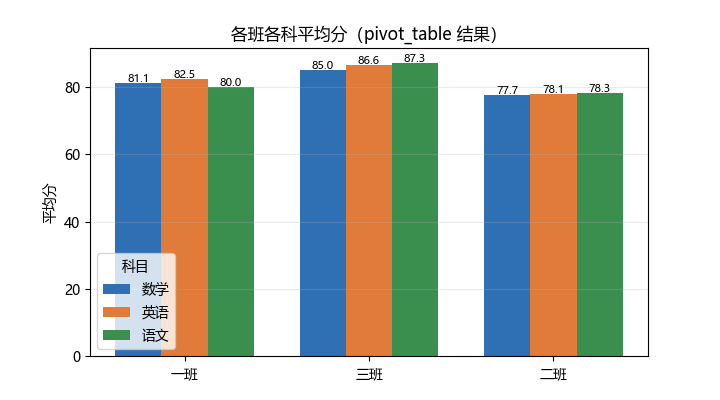
\includegraphics[keepaspectratio,alt={各班各科平均分}]{figures/04-pandas/case_scores.png}}
\caption{各班各科平均分}
\end{figure}

绘图代码：

\begin{Shaded}
\begin{Highlighting}[]
\ImportTok{import}\NormalTok{ matplotlib.pyplot }\ImportTok{as}\NormalTok{ plt}
\NormalTok{plt.rcParams[}\StringTok{\textquotesingle{}font.sans{-}serif\textquotesingle{}}\NormalTok{] }\OperatorTok{=}\NormalTok{ [}\StringTok{\textquotesingle{}Microsoft YaHei\textquotesingle{}}\NormalTok{, }\StringTok{\textquotesingle{}SimHei\textquotesingle{}}\NormalTok{, }\StringTok{\textquotesingle{}DejaVu Sans\textquotesingle{}}\NormalTok{]}
\NormalTok{plt.rcParams[}\StringTok{\textquotesingle{}axes.unicode\_minus\textquotesingle{}}\NormalTok{] }\OperatorTok{=} \VariableTok{False}

\NormalTok{fig, ax }\OperatorTok{=}\NormalTok{ plt.subplots(figsize}\OperatorTok{=}\NormalTok{(}\FloatTok{7.2}\NormalTok{, }\FloatTok{4.0}\NormalTok{))}
\NormalTok{subjects }\OperatorTok{=}\NormalTok{ piv.columns.tolist()}
\NormalTok{x }\OperatorTok{=}\NormalTok{ np.arange(}\BuiltInTok{len}\NormalTok{(piv.index))}
\NormalTok{colors }\OperatorTok{=}\NormalTok{ [}\StringTok{\textquotesingle{}\#2f6fb3\textquotesingle{}}\NormalTok{, }\StringTok{\textquotesingle{}\#e07b39\textquotesingle{}}\NormalTok{, }\StringTok{\textquotesingle{}\#3a8f4f\textquotesingle{}}\NormalTok{]}
\ControlFlowTok{for}\NormalTok{ j, sub }\KeywordTok{in} \BuiltInTok{enumerate}\NormalTok{(subjects):}
\NormalTok{    vals }\OperatorTok{=}\NormalTok{ piv[sub].values}
\NormalTok{    ax.bar(x }\OperatorTok{+}\NormalTok{ (j }\OperatorTok{{-}} \DecValTok{1}\NormalTok{) }\OperatorTok{*} \FloatTok{0.25}\NormalTok{, vals, width}\OperatorTok{=}\FloatTok{0.25}\NormalTok{, label}\OperatorTok{=}\NormalTok{sub, color}\OperatorTok{=}\NormalTok{colors[j])}
    \ControlFlowTok{for}\NormalTok{ xi, v }\KeywordTok{in} \BuiltInTok{zip}\NormalTok{(x }\OperatorTok{+}\NormalTok{ (j }\OperatorTok{{-}} \DecValTok{1}\NormalTok{) }\OperatorTok{*} \FloatTok{0.25}\NormalTok{, vals):}
\NormalTok{        ax.text(xi, v }\OperatorTok{+} \FloatTok{0.3}\NormalTok{, }\SpecialStringTok{f\textquotesingle{}}\SpecialCharTok{\{}\NormalTok{v}\SpecialCharTok{:.1f\}}\SpecialStringTok{\textquotesingle{}}\NormalTok{, ha}\OperatorTok{=}\StringTok{\textquotesingle{}center\textquotesingle{}}\NormalTok{, fontsize}\OperatorTok{=}\DecValTok{8}\NormalTok{)}
\NormalTok{ax.set\_xticks(x)}
\NormalTok{ax.set\_xticklabels(piv.index)}
\NormalTok{ax.set\_ylabel(}\StringTok{\textquotesingle{}平均分\textquotesingle{}}\NormalTok{)}
\NormalTok{ax.set\_title(}\StringTok{\textquotesingle{}各班各科平均分（pivot\_table 结果）\textquotesingle{}}\NormalTok{)}
\NormalTok{ax.legend(title}\OperatorTok{=}\StringTok{\textquotesingle{}科目\textquotesingle{}}\NormalTok{)}
\NormalTok{ax.grid(axis}\OperatorTok{=}\StringTok{\textquotesingle{}y\textquotesingle{}}\NormalTok{, alpha}\OperatorTok{=}\FloatTok{0.25}\NormalTok{)}
\NormalTok{fig.savefig(}\StringTok{\textquotesingle{}figures/04{-}pandas/case\_scores.png\textquotesingle{}}\NormalTok{)}
\NormalTok{plt.close(fig)}
\end{Highlighting}
\end{Shaded}

\subsubsection{4.2
各班成绩分布直方图}\label{ux5404ux73edux6210ux7ee9ux5206ux5e03ux76f4ux65b9ux56fe}

\begin{figure}
\centering
\pandocbounded{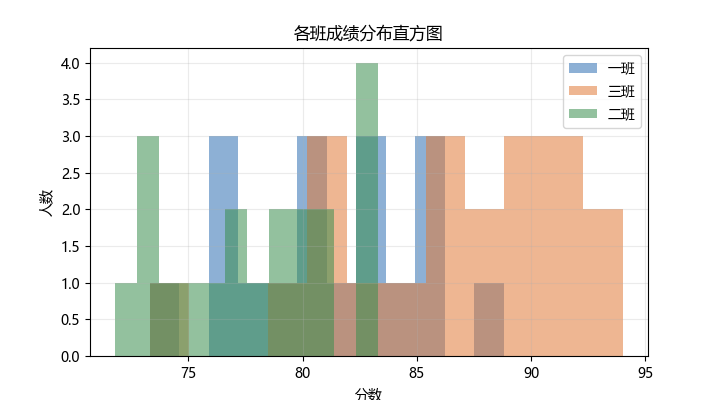
\includegraphics[keepaspectratio,alt={各班成绩分布}]{figures/04-pandas/case_distribution.png}}
\caption{各班成绩分布}
\end{figure}

\begin{Shaded}
\begin{Highlighting}[]
\NormalTok{fig, ax }\OperatorTok{=}\NormalTok{ plt.subplots(figsize}\OperatorTok{=}\NormalTok{(}\FloatTok{7.2}\NormalTok{, }\FloatTok{4.0}\NormalTok{))}
\ControlFlowTok{for}\NormalTok{ (cls, g), c }\KeywordTok{in} \BuiltInTok{zip}\NormalTok{(df.groupby(}\StringTok{\textquotesingle{}班级\textquotesingle{}}\NormalTok{), colors):}
\NormalTok{    ax.hist(g[}\StringTok{\textquotesingle{}分数\textquotesingle{}}\NormalTok{], bins}\OperatorTok{=}\DecValTok{12}\NormalTok{, alpha}\OperatorTok{=}\FloatTok{0.55}\NormalTok{, label}\OperatorTok{=}\NormalTok{cls, color}\OperatorTok{=}\NormalTok{c)}
\NormalTok{ax.set\_xlabel(}\StringTok{\textquotesingle{}分数\textquotesingle{}}\NormalTok{)}
\NormalTok{ax.set\_ylabel(}\StringTok{\textquotesingle{}人数\textquotesingle{}}\NormalTok{)}
\NormalTok{ax.set\_title(}\StringTok{\textquotesingle{}各班成绩分布直方图\textquotesingle{}}\NormalTok{)}
\NormalTok{ax.legend()}
\NormalTok{ax.grid(alpha}\OperatorTok{=}\FloatTok{0.25}\NormalTok{)}
\NormalTok{fig.savefig(}\StringTok{\textquotesingle{}figures/04{-}pandas/case\_distribution.png\textquotesingle{}}\NormalTok{)}
\NormalTok{plt.close(fig)}
\end{Highlighting}
\end{Shaded}

\subsubsection{4.3 时间序列：日到课人数 →
周均与移动平均}\label{ux65f6ux95f4ux5e8fux5217ux65e5ux5230ux8bfeux4ebaux6570-ux5468ux5747ux4e0eux79fbux52a8ux5e73ux5747}

\begin{figure}
\centering
\pandocbounded{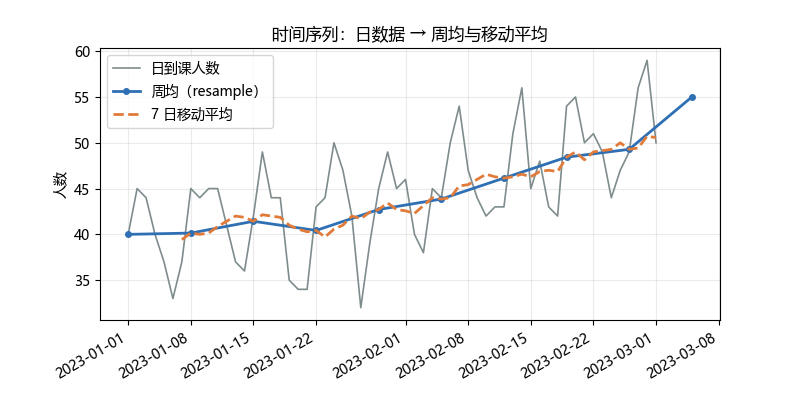
\includegraphics[keepaspectratio,alt={时间序列}]{figures/04-pandas/case_time_series.png}}
\caption{时间序列}
\end{figure}

\begin{Shaded}
\begin{Highlighting}[]
\NormalTok{rng }\OperatorTok{=}\NormalTok{ np.random.default\_rng(}\DecValTok{7}\NormalTok{)}
\NormalTok{idx }\OperatorTok{=}\NormalTok{ pd.date\_range(}\StringTok{\textquotesingle{}2023{-}01{-}01\textquotesingle{}}\NormalTok{, periods}\OperatorTok{=}\DecValTok{60}\NormalTok{, freq}\OperatorTok{=}\StringTok{\textquotesingle{}D\textquotesingle{}}\NormalTok{)}
\NormalTok{trend }\OperatorTok{=}\NormalTok{ np.linspace(}\DecValTok{0}\NormalTok{, }\DecValTok{10}\NormalTok{, }\DecValTok{60}\NormalTok{)}
\NormalTok{weekly }\OperatorTok{=} \DecValTok{5} \OperatorTok{*}\NormalTok{ np.sin(}\DecValTok{2} \OperatorTok{*}\NormalTok{ np.pi }\OperatorTok{*}\NormalTok{ np.arange(}\DecValTok{60}\NormalTok{) }\OperatorTok{/} \DecValTok{7}\NormalTok{)}
\NormalTok{count }\OperatorTok{=}\NormalTok{ (}\DecValTok{40} \OperatorTok{+}\NormalTok{ trend }\OperatorTok{+}\NormalTok{ weekly }\OperatorTok{+}\NormalTok{ rng.normal(}\DecValTok{0}\NormalTok{, }\DecValTok{3}\NormalTok{, }\DecValTok{60}\NormalTok{)).}\BuiltInTok{round}\NormalTok{().clip(}\DecValTok{0}\NormalTok{, }\DecValTok{60}\NormalTok{).astype(}\BuiltInTok{int}\NormalTok{)}
\NormalTok{ts }\OperatorTok{=}\NormalTok{ pd.Series(count, index}\OperatorTok{=}\NormalTok{idx)}
\NormalTok{weekly\_mean }\OperatorTok{=}\NormalTok{ ts.resample(}\StringTok{\textquotesingle{}W\textquotesingle{}}\NormalTok{).mean()}
\NormalTok{rolling7 }\OperatorTok{=}\NormalTok{ ts.rolling(}\DecValTok{7}\NormalTok{).mean()}

\NormalTok{fig, ax }\OperatorTok{=}\NormalTok{ plt.subplots(figsize}\OperatorTok{=}\NormalTok{(}\FloatTok{8.0}\NormalTok{, }\FloatTok{4.0}\NormalTok{))}
\NormalTok{ax.plot(ts.index, ts.values, color}\OperatorTok{=}\StringTok{\textquotesingle{}\#7f8c8d\textquotesingle{}}\NormalTok{, lw}\OperatorTok{=}\FloatTok{1.2}\NormalTok{, label}\OperatorTok{=}\StringTok{\textquotesingle{}日到课人数\textquotesingle{}}\NormalTok{)}
\NormalTok{ax.plot(weekly\_mean.index, weekly\_mean.values, color}\OperatorTok{=}\StringTok{\textquotesingle{}\#2f6fb3\textquotesingle{}}\NormalTok{, marker}\OperatorTok{=}\StringTok{\textquotesingle{}o\textquotesingle{}}\NormalTok{, ms}\OperatorTok{=}\DecValTok{4}\NormalTok{,}
\NormalTok{        lw}\OperatorTok{=}\DecValTok{2}\NormalTok{, label}\OperatorTok{=}\StringTok{\textquotesingle{}周均（resample）\textquotesingle{}}\NormalTok{)}
\NormalTok{ax.plot(rolling7.index, rolling7.values, color}\OperatorTok{=}\StringTok{\textquotesingle{}\#e07b39\textquotesingle{}}\NormalTok{, lw}\OperatorTok{=}\DecValTok{2}\NormalTok{, ls}\OperatorTok{=}\StringTok{\textquotesingle{}{-}{-}\textquotesingle{}}\NormalTok{, label}\OperatorTok{=}\StringTok{\textquotesingle{}7 日移动平均\textquotesingle{}}\NormalTok{)}
\NormalTok{ax.set\_ylabel(}\StringTok{\textquotesingle{}人数\textquotesingle{}}\NormalTok{)}
\NormalTok{ax.set\_title(}\StringTok{\textquotesingle{}时间序列：日数据 → 周均与移动平均\textquotesingle{}}\NormalTok{)}
\NormalTok{ax.legend()}
\NormalTok{ax.grid(alpha}\OperatorTok{=}\FloatTok{0.25}\NormalTok{)}
\NormalTok{fig.autofmt\_xdate()}
\NormalTok{fig.savefig(}\StringTok{\textquotesingle{}figures/04{-}pandas/case\_time\_series.png\textquotesingle{}}\NormalTok{)}
\NormalTok{plt.close(fig)}
\end{Highlighting}
\end{Shaded}

\subsection{5. 结论}\label{ux7ed3ux8bba}

\begin{itemize}
\tightlist
\item
  清洗后共 58 条有效记录，去掉 2 个缺失、1 行重复，并用 IQR 替换了 1
  个异常低分；
\item
  三班平均分最高（86.3），二班最低（78.0），这与我们设定的``班级基础分''一致；
\item
  透视表给出``班级 × 科目''的平均分，能快速定位薄弱科目；
\item
  时间序列图说明：\texttt{resample(\textquotesingle{}W\textquotesingle{})}
  把日数据聚合成周均，\texttt{rolling(7)} 得到平滑的 7
  日移动平均，二者都可用于观察趋势。
\end{itemize}

\subsection{拓展任务}\label{ux62d3ux5c55ux4efbux52a1-6}

\begin{enumerate}
\def\labelenumi{\arabic{enumi}.}
\tightlist
\item
  改用真实 CSV（如某课程成绩表）复现；
\item
  把
  \texttt{groupby(\textquotesingle{}班级\textquotesingle{}){[}\textquotesingle{}分数\textquotesingle{}{]}.agg({[}\textquotesingle{}mean\textquotesingle{},\ \textquotesingle{}std\textquotesingle{},\ \textquotesingle{}count\textquotesingle{}{]})}
  的结果也画成条形图；
\item
  对透视表加 \texttt{margins=True} 显示总计；
\item
  给时间序列数据加周末标记，观察周末到课人数是否更低。
\end{enumerate}

\subsection{延伸阅读}\label{ux5ef6ux4f38ux9605ux8bfb-19}

\begin{itemize}
\tightlist
\item
  Pandas
  分组与聚合文档：https://pandas.pydata.org/docs/user\_guide/groupby.html
\item
  Pandas
  透视表文档：https://pandas.pydata.org/docs/reference/api/pandas.pivot\_table.html
\item
  Pandas
  时间序列文档：https://pandas.pydata.org/docs/user\_guide/timeseries.html
\item
  Matplotlib
  官方入门：https://matplotlib.org/stable/tutorials/introductory/quick\_start.html
\end{itemize}

\section{04
常见误区与技巧}\label{ux5e38ux89c1ux8befux533aux4e0eux6280ux5de7-3}

\begin{quote}
本章为新增``查漏补缺''页：把学生最容易踩的坑集中列出，并给出正确的写法和性能/调试建议。
\end{quote}

\subsection{1.
高频误区速查表}\label{ux9ad8ux9891ux8befux533aux901fux67e5ux8868-3}

{\def\LTcaptype{none} % do not increment counter
\begin{longtable}[]{@{}
  >{\raggedright\arraybackslash}p{(\linewidth - 6\tabcolsep) * \real{0.2500}}
  >{\raggedright\arraybackslash}p{(\linewidth - 6\tabcolsep) * \real{0.2500}}
  >{\raggedright\arraybackslash}p{(\linewidth - 6\tabcolsep) * \real{0.2500}}
  >{\raggedright\arraybackslash}p{(\linewidth - 6\tabcolsep) * \real{0.2500}}@{}}
\toprule\noalign{}
\begin{minipage}[b]{\linewidth}\raggedright
\#
\end{minipage} & \begin{minipage}[b]{\linewidth}\raggedright
误区 / 错误写法
\end{minipage} & \begin{minipage}[b]{\linewidth}\raggedright
正确做法
\end{minipage} & \begin{minipage}[b]{\linewidth}\raggedright
原因
\end{minipage} \\
\midrule\noalign{}
\endhead
\bottomrule\noalign{}
\endlastfoot
1 & \texttt{df.loc{[}0{]}} 想取第一行但索引是字符串 &
\texttt{df.iloc{[}0{]}}（位置）或
\texttt{df.loc{[}\textquotesingle{}r0\textquotesingle{}{]}}（标签） &
loc 按标签、iloc 按位置 \\
2 & \texttt{s{[}0{]}} 取 Series 位置 & \texttt{s.iloc{[}0{]}} &
整数标签歧义，位置访问应显式 iloc \\
3 & \texttt{df{[}(df.A\textgreater{}2)\ and\ (df.B\textless{}40){]}} &
\texttt{df{[}(df.A\textgreater{}2)\ \&\ (df.B\textless{}40){]}}（每个条件加括号）
& \texttt{and}/\texttt{or} 用于 Python
布尔，\texttt{\&}/\texttt{\textbar{}} 用于逐元素布尔数组 \\
4 & \texttt{df{[}\textquotesingle{}A\textquotesingle{}{]}} 当``单个
DataFrame'' & 需要单列 DataFrame 用
\texttt{df{[}{[}\textquotesingle{}A\textquotesingle{}{]}{]}} &
\texttt{df{[}\textquotesingle{}A\textquotesingle{}{]}} 返回 Series \\
5 & \texttt{fillna(method=\textquotesingle{}ffill\textquotesingle{})} &
\texttt{df.ffill()} & pandas 2.x 已弃用 method 写法 \\
6 & \texttt{dropna()} 误删有效数据 & 先 \texttt{df.isna().sum()}
看缺失情况，用 \texttt{thresh} 控制 & dropna 默认删任意含缺失的行 \\
7 & 以为 \texttt{groupby} 返回 DataFrame & 返回 \texttt{groupby}
对象，需 \texttt{.mean()}/\texttt{.agg()} 等 & groupby 是``中间对象'' \\
8 & \texttt{pivot\_table} 出现 NaN & 加 \texttt{fill\_value=0} &
交叉格无数据 \\
9 & \texttt{resample(\textquotesingle{}W\textquotesingle{})}
当``滑动平均'' & 降频聚合用 resample；滑窗用 \texttt{rolling(7).mean()}
& 二者语义不同 \\
10 & 用 \texttt{apply} 做可向量化运算 & \texttt{s*2+1} 优先 & apply 逐行
Python 调用，慢 \\
11 & 修改切片后以为原数据不变 & 注意 Pandas
的视图/拷贝语义（建议对新结果 \texttt{.copy()}） & 部分切片是视图 \\
12 & 读 Excel 报错 & 先 \texttt{pip\ install\ openpyxl} & 缺读写引擎 \\
\end{longtable}
}

\subsection{2. 原理级难点：loc vs
iloc}\label{ux539fux7406ux7ea7ux96beux70b9loc-vs-iloc}

\begin{Shaded}
\begin{Highlighting}[]
\NormalTok{s }\OperatorTok{=}\NormalTok{ pd.Series([}\DecValTok{10}\NormalTok{, }\DecValTok{20}\NormalTok{, }\DecValTok{30}\NormalTok{], index}\OperatorTok{=}\NormalTok{[}\StringTok{\textquotesingle{}a\textquotesingle{}}\NormalTok{, }\StringTok{\textquotesingle{}b\textquotesingle{}}\NormalTok{, }\StringTok{\textquotesingle{}c\textquotesingle{}}\NormalTok{])}
\BuiltInTok{print}\NormalTok{(s.loc[}\StringTok{\textquotesingle{}b\textquotesingle{}}\NormalTok{])     }\CommentTok{\# 20（按标签）}
\BuiltInTok{print}\NormalTok{(s.iloc[}\DecValTok{1}\NormalTok{])      }\CommentTok{\# 20（按位置）}
\end{Highlighting}
\end{Shaded}

\begin{itemize}
\tightlist
\item
  标签是字符串时，\texttt{s{[}0{]}} 会歧义甚至报错；统一
  \texttt{s.loc{[}\textquotesingle{}b\textquotesingle{}{]}} /
  \texttt{s.iloc{[}1{]}}。
\item
  \texttt{.loc}
  切片是\textbf{闭区间}（\texttt{df.loc{[}\textquotesingle{}a\textquotesingle{}:\textquotesingle{}c\textquotesingle{}{]}}
  含 c），\texttt{.iloc}
  切片是\textbf{开区间}（\texttt{df.iloc{[}0:2{]}} 只含 0,1）。
\end{itemize}

\subsection{3. 性能技巧}\label{ux6027ux80fdux6280ux5de7-3}

\begin{itemize}
\tightlist
\item
  \textbf{向量化优先}：能
  \texttt{df{[}\textquotesingle{}x\textquotesingle{}{]}\ *\ 2\ +\ 1}
  就不要
  \texttt{df{[}\textquotesingle{}x\textquotesingle{}{]}.apply(lambda\ v:\ v*2+1)}；
\item
  \textbf{避免在循环里逐行
  \texttt{append}/\texttt{concat}}：先用列表收集再一次性
  \texttt{pd.DataFrame(...)}；
\item
  \textbf{用 \texttt{rename}/\texttt{astype}
  前先想好副本}：多数方法返回新对象；
\item
  \textbf{大文件用
  \texttt{chunksize}}：\texttt{pd.read\_csv(\textquotesingle{}big.csv\textquotesingle{},\ chunksize=10\_000)}
  分批读；
\item
  \textbf{时间序列避免逐元素循环}：用
  \texttt{resample}/\texttt{rolling}/\texttt{shift}/\texttt{diff}；
\item
  \textbf{用 \texttt{pd.qcut}/\texttt{cut}} 做分箱，避免手写条件判断。
\end{itemize}

\subsection{4. 调试建议}\label{ux8c03ux8bd5ux5efaux8bae-3}

\begin{enumerate}
\def\labelenumi{\arabic{enumi}.}
\tightlist
\item
  先打印 \texttt{df.head()}、\texttt{df.dtypes}、\texttt{df.shape}
  确认数据形状；
\item
  布尔筛选把中间掩码存成变量：\texttt{mask\ =\ (df.A\ \textgreater{}\ 2)\ \&\ (df.B\ \textless{}\ 40);\ df{[}mask{]}}；
\item
  用 \texttt{df.isna().sum()} 检查缺失；用
  \texttt{df.duplicated().sum()} 检查重复；
\item
  遇到 \texttt{KeyError} 先打印 \texttt{df.columns}；
\item
  数值异常用 \texttt{df.describe()} 看 min/max/分位数；
\item
  随机/抽样问题\textbf{固定种子}
  \texttt{rng\ =\ np.random.default\_rng(42)}。
\end{enumerate}

\subsection{5.
本章小结（自测清单）}\label{ux672cux7ae0ux5c0fux7ed3ux81eaux6d4bux6e05ux5355}

\begin{itemize}
\tightlist
\item[$\square$]
  能解释 Series 与 DataFrame 的区别；
\item[$\square$]
  能说出 \texttt{.loc} 与 \texttt{.iloc} 的三个不同点；
\item[$\square$]
  会写 \texttt{df{[}(df.A\textgreater{}2)\ \&\ (df.B\textless{}40){]}}
  的多条件布尔筛选；
\item[$\square$]
  会用
  \texttt{drop\_duplicates}/\texttt{fillna}/\texttt{dropna}/\texttt{ffill}
  清数据；
\item[$\square$]
  会用 IQR 找异常并替换；
\item[$\square$]
  会做 Min-Max 与 Z-Score，并说出适用场景；
\item[$\square$]
  会 \texttt{groupby}/\texttt{pivot\_table} 做分组透视；
\item[$\square$]
  会 \texttt{resample}/\texttt{rolling} 处理时间序列；
\item[$\square$]
  会画 matplotlib 图（中文字体）并生成案例配图。
\end{itemize}

\subsection{延伸阅读}\label{ux5ef6ux4f38ux9605ux8bfb-20}

\begin{itemize}
\tightlist
\item
  Pandas
  官方``用户指南''：https://pandas.pydata.org/docs/user\_guide/index.html
\item
  Pandas
  官方``性能提升''：https://pandas.pydata.org/docs/user\_guide/enhancingperf.html
\item
  Python Data Science Handbook（第 3 章
  Pandas）：https://github.com/jakevdp/PythonDataScienceHandbook
\end{itemize}

\newpage
